Uno de los principales problemas de hacer ingeniería de rendimiento para software en la nube es que no existen aplicaciones de referencia que hayan ganado popularidad o cuyo desarrollo se encuentre activo. A pesar de esto y de su reciente adopción, la industria ha empezado a reconocer casos de uso en donde las aplicaciones \emph{serverless} encajan mejor. Amazon Web Services(AWS)\cite{serverless-architecture-patterns} reconoce cinco patrones de uso predominantes en su servicio AWS Lambda:
\begin{enumerate}
    \item Procesamiento de datos dirigidos por eventos.
    \item Aplicaciones Web.
    \item Aplicaciones móviles e Internet las cosas (IoT).
    \item Ecosistemas de aplicaciones \emph{serverless}.
    \item Flujos de trabajo dirigidos por eventos.
\end{enumerate}
 
Uno de las aplicaciones más comunes en \emph{serverless} es desencadenar acciones luego de que ocurre un evento (1), por ejemplo luego de la modificación de un registro en una base de datos o bien luego de que se publica un mensaje en una cola de mensajería. Esto puede provocar que se active una función Lambda\footnote{En la plataforma AWS Lambda } que toma como entrada el evento recién publicado para su posterior procesamiento. Este estilo de caso de uso encaja bien en ambientes híbridos: ambientes en donde tecnologías \emph{serverless} se aprovechan para realizar funciones específicas dentro de una aplicación (o aplicaciones) más grande.

AWS ha publicado una serie de arquitecturas de referencia\cite{aws-lambda-ref-arch} para su plataforma FaaS, AWS Lambda. Dentro de estas arquitecturas se destaca el caso de uso de un manejador de imágenes (\emph{Image Handler})\cite{aws-lambda-image-handler}. 

\begin{figure}[h]
  \centering
  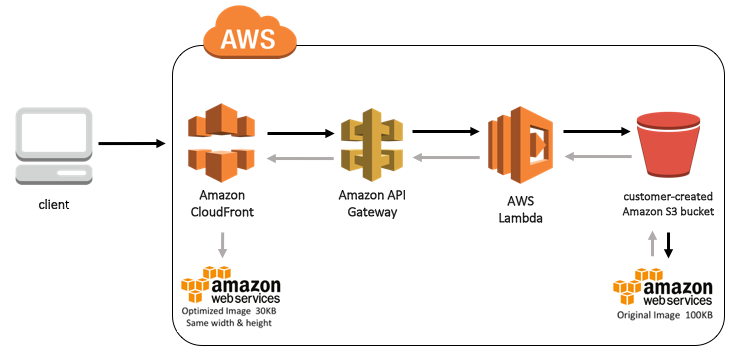
\includegraphics[width=15cm]{serverless-image-handler-architecture}
  \caption[Arquitectura del manejador de imágenes]{Arquitectura del manejador de imágenes. Tomado de \protect\cite{aws-lambda-image-handler}}
  \label{fig:serverless-image-handler-architecture}
\end{figure}

\section{\emph{Manejador de imágenes}} \label{sec:manejador-imagenes-1}
Sitios Web con imágenes grandes pueden experimentar tiempos de carga prolongados, es por esto que los desarrolladores proporcionan diferentes versiones de cada imagen para que se acomoden a distintos anchos de banda o diseños de página. Para brindar tiempos de respuesta cortos y disminuir el costo de la optimización, manipulación y procesamiento de las imágenes, AWS propone un manejador de imágenes \emph{serverless}, al cual se le pueda delegar tal trabajo como una función Lambda sobre la plataforma FaaS.


A continuación se describe la arquitectura de la figura \ref{fig:serverless-image-handler-architecture}:
\begin{enumerate}
    \item Amazon CloudFront provee una capa de \emph{cache} para reducir el costo del procesamiento de la imagen
    \item Amazon API Gateway brinda acceso por medio de HTTP a las funciones Lambda
    \item AWS Lambda obtiene la imagen de un repositorio de Amazon Simple Storage Service (Amazon S3) y por medio de la implementación de la función se retorna una versión modificada de la imagen al API Gateway
    \item El API Gateway retorna una nueva imagen a CloudFront para su posterior entrega a los usuarios finales
\end{enumerate}

Cabe mencionar que, en este contexto, una versión modificada de una imagen será cualquier imagen que haya presentado algún tipo de alteración con respeto de una imagen original como, por ejemplo, cambios de tamaño, color, metadatos, etc.

\subsection{Manejador de imágenes para SPE} \label{sec:manejador-imagenes-spe}
Para este estudio se proponemos implementar una variación del manejador de imágenes de la sección \ref{sec:manejador-imagenes-1}, que se muestra en la figura \ref{fig:serverless-image-handler-architecture-spe}.

\begin{figure}[h]
  \centering
  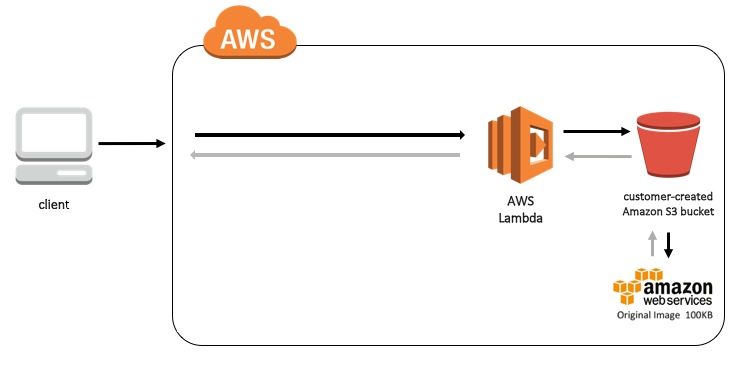
\includegraphics[width=15cm]{serverless-image-handler-architecture-spe}
  \caption[Arquitectura del manejador de imágenes propuesto para el estudio]{Arquitectura del manejador de imágenes propuesto para el estudio.}
  \label{fig:serverless-image-handler-architecture-spe}
\end{figure}

Se han dejado por fuera intencionalmente el AWS CloudFront y el AWS API Gateway. La razón de esto es porque se pretende ejercitar la función Lambda directamente. Se implementará una función Lambda que entregue a partir de una solicitud de redimensionamiento de una imagen almacenada, otra con dimensiones diferentes producida ``al vuelo'' como respuesta a la solicitud. Por ejemplo, si la imagen original mide 500 pixeles de ancho y alto, entregar una con dimensiones de 100 pixeles de ancho y alto. 

Las actividades involucradas en el proceso de redimensionamientos de imágenes se muestran en la figura \ref{fig:serverless-image-handler-architecture-workflow}
\begin{enumerate}
    \item Se envía una solicitud de redimensionamiento de imagen en formato \texttt{JSON} a la función Lambda con los datos acerca de la localización de la imagen y su nuevo tamaño.
    \item La solicitud de redimensionamiento llega a la función Lambda.
    \item La función Lambda solicita al servicio de almacemiento AWS S3 la imagen.
    \item AWS S3 entrega a la función Lambda la imagen solicitada.
    \item La función Lambda inicia el redimensionamiento de la imagen de acuerdo a los parámetros solicitados.
    \item La nueva imagen modificada se entrega al cliente(s).
\end{enumerate}

\begin{figure}[h]
  \centering
  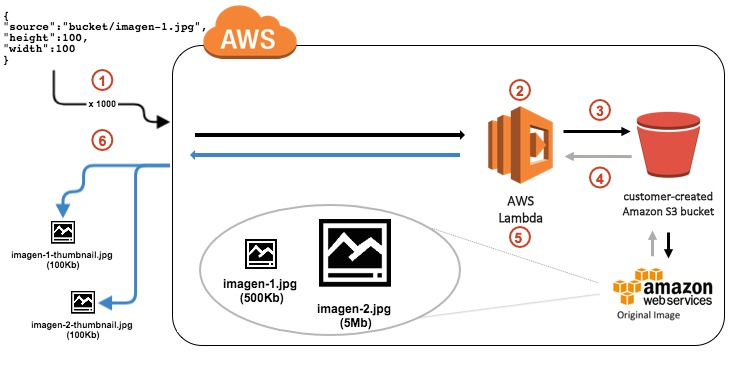
\includegraphics[width=17cm]{serverless-image-handler-architecture-workflow-2}
  \caption[Carga de trabajo sugerida para el manejador de imágenes]{Carga de trabajo sugerida para el manejador de imágenes}
  \label{fig:serverless-image-handler-architecture-workflow}
\end{figure}


A la función Lambda se le realizarán pruebas con imágenes de entrada de distinto tamaño y cargas de trabajo variables para evaluar su comportamiento bajo estos escenarios. Se desea observar el impacto de las pruebas en el tiempo de respuesta de la función. Los resultados obtenidos a partir de estas pruebas van a servir como un punto de referencia para experimentos futuros, como los que se indican en la Sección \ref{sec:experimentos-propuestos}. La figura \ref{fig:serverless-image-handler-architecture-workflow} muestra una sugerencia de dos posibles cargas de trabajo: 

\begin{enumerate}
    \item 100 solicitudes de cambio de tamaño de una imagen grande. En la figura \ref{fig:serverless-image-handler-architecture-workflow}, \texttt{imagen-2.jpg} de tamaño de 5Mb, representa una imagen grande.
    \item 100 solicitudes de cambio de tamaño de una imagen pequeña. En la figura \ref{fig:serverless-image-handler-architecture-workflow}, \texttt{imagen-1.jpg} de tamaño menor o igual a 500Kb, representa una imagen pequeña.
\end{enumerate}

En principio las cargas de trabajo generadas serían \emph{cerradas}, lo que quiere decir que una solicitud se ejecuta solamente hasta que la anterior se termina. Esto ayudará en principio a tener mejor trazabilidad de lo que ocurre con la función.

\paragraph{¿Por qué este caso de uso se considera relevante?}
A continuación se listan las características que hacen este caso de uso representativo e interesante:
\begin{itemize}
    \item Sencillo de entender e implementar: se cuenta únicamente con una función la cual lleva a cabo una tarea muy específica.
    \item Popular: sigue un patrón de procesamiento dirigido por eventos y, como se señala en \cite{serverless-architecture-patterns}, este es uno de los más populares que se ha empezado a adoptar para aplicaciones \emph{serverless}. Otra de las razones de la popularidad de este caso de uso es que permite a los desarrolladores crear una unidad de instalación independiente y especializada para el manejo de imágenes, liberando así a sus servidores y aplicaciones del manejo de las peticiones y lógica asociadas a estas.
    \item Replicable en otros proveedores de servicios en la nube: varias de las arquitecturas de referencia para \emph{serverless} propuestas por Amazon, están compuestas por herramientas y servicios muy propios de su plataforma, lo cual hace muy difícil su reproducibilidad utilizando otros proveedores. Aunque en principio este trabajo plantea ser elaborado en la plataforma FaaS de Amazon Web Services, AWS Lambda, otros proveedores de servicios (ver sección \ref{sec:proveedores-faas}) en la nube cuentan con sus propias plataformas de FaaS y de almacenamiento, lo cual permitiría replicar lo aquí propuesto en ellos.
    \item Replicable en los lenguajes de programación soportados por plataformas FaaS: actualmente JavaScript, Java (y lenguajes basados en la \emph{Java Virtual Machine}), Python, C\# y Go son los principales lenguajes de programación soportados por las plataformas FaaS. El caso de uso propuesto, no presenta ningún tipo de característica que lo ate a un lenguaje de programación en particular. En todos ellos se cuentan con bibliotecas para manejo de imágenes tanto de forma nativa como por medio de soluciones de terceros. 
\end{itemize}


\section{Implementación del \emph{manejador de imágenes}}
Existen soluciones disponibles que se pueden estudiar para implementar un manejador de imágenes. Amazon proporciona dos ejemplos que siguen la arquitectura de la figura \ref{fig:serverless-image-handler-architecture}:
\begin{enumerate}
    \item \textbf{{serverless-image-resizing}}\footnote{\url{https://github.com/amazon-archives/serverless-image-resizing}}: escrita en lenguaje JavaScript. Utiliza el modulo \emph{sharp}\footnote{\url{https://github.com/lovell/sharp}} de NodeJS para aplicar operaciones de conversión en imágenes tales como redimensionamiento, rotación y corrección gamma.
    \item \textbf{{serverless-image-handler}}\footnote{\url{https://github.com/awslabs/serverless-image-handler}}: escrita en lenguaje Python. Hace uso del paquete \emph{Thumbor}\footnote{\url{http://thumbor.org}} de código abierto para realizar operaciones de redimensionamiento, rotación, recorte y aplicación de filtros en imágenes.
\end{enumerate}

A pesar que Amazon recomienda el uso de \emph{serverless-image-handler} sobre \emph{serverless-image-resizing}, ambas soluciones siguen un patrón sumamente similar en su codificación e instalación. 

Otro ejemplo de una función en la nube encargada de ofrecer un servicio de redimensionamiento en imágenes, es la \emph{Course\_LambdaResizer}, una función lambda usada como referencia en el curso \emph{``Serverless API on AWS for Java developers''} ofrecido en el sitio Web Udemy\footnote{\url{https://www.udemy.com/serverless-api-aws-lambda-for-java-developers}}. Esta función está escrita en lenguaje Java y utiliza la biblioteca \emph{imgscalr}\footnote{\url{https://github.com/rkalla/imgscalr}} para redimensionar imágenes.

Para este estudio, se implementó una función escrita en lenguaje Java. Esto motivado principalmente por la compatibilidad de este lenguaje con las herramientas para monitoreo de aplicaciones y extracción de modelos de rendimiento, Kieker y PMX respectivamente.

\subsection{Función Lambda: \emph{Image-Handler} (IM-Simple)}\label{sec:image-handler}
La función Lambda creada para este estudio lleva por nombre \emph{Image-Handler}. El código fuente y documentación relacionada con la misma se encuentra disponible en GitHub.com, en el repositorio de código: \url{https://github.com/seminario-dos/image-handler}. El punto de entrada de la función Lambda es la clase \texttt{ImageHandler.java}. Esta función se encarga de realizar tres operaciones para procesar una solicitud de redimensionamiento de imagen:

\begin{enumerate}
    \item Procesar la solicitud de redimiensionamiento (la entrada) que viene dada en formato JSON. Esta solicitud de redimensionamiento contiene entre otras cosas:
    \begin{itemize}
        \item El nombre de la imagen original que reside en el servicio Amazon S3.
        \item Los parámetros de altura y ancho a los que se desea redimensionar la imagen original.
    \end{itemize}
    \item Obtener la imagen del servicio Amazon S3 y posteriormente aplicar la operación de redimiensionamiento sobre la misma de acuerdo a los parámetros de altura y ancho especificados en la solicitud de redimensionamiento.
    \item Tomar la imagen redimensionada, codificarla en \texttt{Base64} y escribir el resultado en el flujo(\emph{stream}) de salida de la función Lambda.
\end{enumerate}
 
Un extracto de la clase \texttt{ImageHandler.java} se muestra en el listado \ref{lst:lambda-1}. En la línea \texttt{22} se procesa el evento de entrada que viene dado en formato JSON. Como resultado de esto se entrega un objeto \texttt{ImageRequest} el cual contiene la información de la solicitud de la imagen que se desea redimensionar y que se encuentra alojada en el servicio Amazon S3.

En la línea \texttt{24} se llama al servicio \texttt{ImageService} con el fin de obtener la imagen   original (de acuerdo a la información presente en el \texttt{ImageRequest} proporcionado) y se aplica la operación de redimensionamiento.

Por último, en la línea \texttt{26}, \texttt{ImageHandlerResponseWriter.writeResponse()} toma la nueva imagen, con nuevas dimensiones de alto y ancho, la codifica en \texttt{Base64} y escribe el resultado en el \emph{stream} de salida de la función. 

\begin{lstlisting}[linewidth=16.5cm, caption={Clase \texttt{ImageHandler.java}}, label={lst:lambda-1}]
public class ImageHandler implements RequestStreamHandler {

    private static final AppConfig APP_CONFIG;
    private final AppConfig appConfig;

    static {
        APP_CONFIG = AppConfig.getInstance();
    }

    public ImageHandler() {
        this(APP_CONFIG);
    }

    public ImageHandler(AppConfig appConfig) {
        this.appConfig = appConfig;
    }

    @Override
    public void handleRequest(InputStream inputStream, 
                              OutputStream outputStream, 
                              Context context) throws IOException {
        ImageRequest imageRequest = 
            this.inputEventParser().processInputEvent(inputStream);
        InputStream imageResized = 
            this.imageService().getImageFrom(imageRequest);
        this.imageHandlerResponseWriter()
            .writeResponse(imageResized, outputStream, imageRequest);
    }

    private InputEventParser inputEventParser() {
        return this.appConfig.getInputEventParser();
    }

    private ImageService imageService() {
        return this.appConfig.getImageService();
    }

    private ImageHandlerResponseWriter imageHandlerResponseWriter() {
        return this.appConfig.getImageHandlerResponseWriter();
    }
}    
\end{lstlisting}


Las funciones Lambda en AWS reciben como entrada un objeto JSON. Este objeto puede contener distintos campos dependiendo del servicio que haya invocado previamente la ejecución de la función Lambda. Debido a que la función \emph{Image-Handler} pretende ser invocada por medio de solicitudes \texttt{HTTP}, esta se configuró para que trabajara en conjunto con el servicio \texttt{API Gateway}. Dentro de este servicio se creó un recurso Web que entrega solicitudes de tipo \texttt{HTTP GET} a la función Lambda para su posterior procesamiento.

En términos generales, cada vez que una solicitud \texttt{HTTP GET} ingresa al \texttt{API Gateway} con el siguiente formato:\\ \texttt{https://\{host\}/image/\{image\}?width=\{value\}\&height=\{value\}}\\ se tomarán el nombre de la imagen original que viene en el parámetro \texttt{image} y los parámetros de ancho y alto, \texttt{width} y \texttt{height} respectivamente, y se pasarán como parámetros de entrada a la función Lambda como parte de un objeto JSON. Este objeto JSON contiene otros campos que dan a conocer a la función Lambda información acerca de la solicitud \texttt{HTTP}.

\paragraph{Ejemplo:} para la siguiente solicitud \texttt{HTTP}:
\begin{verbatim}
GET https://{host}/images/original-pic.jpg?width=50&height=66
\end{verbatim}

\noindent \texttt{API Gateway} produce el objeto JSON listado en \ref{lst:lambda-api-gateway-input}. A pesar que el objeto JSON incluye otros campos, para efectos del \emph{Image-Handler} solamente tres de ellos serán utilizados:
\begin{enumerate}
    \item \texttt{pathParameters}: contiene el nombre de la imagen original a ser redimensionada.
    \item \texttt{isBase64Encoded}: señala si la solicitud necesita ser codificada en \texttt{Base64} o no. 
    \item \texttt{queryStringParameters}: bajo esta propiedad se listan los parámetros de ancho(\texttt{width}) y alto(\texttt{height}).
\end{enumerate}


\begin{lstlisting}[caption={Clase \texttt{ImageHandler.java}}, label={lst:lambda-api-gateway-input}]
{
  "headers": {
    "Accept": "*/*",
    "User-Agent": "HTTPie/1.0.2",
    "Connection": "keep-alive",
    "X-Forwarded-Proto": "http",
    "Host": "localhost:3000",
    "Accept-Encoding": "gzip, deflate",
    "X-Forwarded-Port": "3000"
  },
  "pathParameters": {
    "image": "original-pic.jpg"
  },
  "path": "/images/original-pic.jpg",
  "isBase64Encoded": true,
  "requestContext": {
    "accountId": "123456789012",
    "path": "/images/{image+}",
    "resourceId": "123456",
    "stage": "prod",
    "requestId": "c6af9ac6-7b61-11e6-9a41-93e8deadbeef",
    "identity": {
      "cognitoIdentityPoolId": null,
      "accountId": null,
      "caller": null,
      "apiKey": null,
      "sourceIp": "127.0.0.1",
      "cognitoAuthenticationType": null,
      "cognitoAuthenticationProvider": null,
      "userArn": null,
      "userAgent": "Custom User Agent String",
      "user": null
    },
    "resourcePath": "/images/{image+}",
    "httpMethod": "GET",
    "extendedRequestId": null,
    "apiId": "1234567890"
  },
  "resource": "/images/{image+}",
  "httpMethod": "GET",
  "body": null,
  "queryStringParameters": {
    "width": "50",
    "height": "66"
  },
  "stageVariables": null
}
\end{lstlisting}

\subsubsection{Principales interacciones dentro de \emph{Image-Handler}}
La figura \ref{fig:secuencia-image-handler} muestra las principales interacciones que lleva a cabo la función \emph{Image-Handler}. Tanto las acciones como los actores involucrados, concuerdan con lo descrito en la Sección \ref{sec:image-handler} aunque, a diferencia de lo descrito allí, aquí se presenta la clase \texttt{S3Dao} que es la que se encarga de buscar y traer la imagen original del servicio Amazon S3. 
\begin{figure}[h]
  \centering
  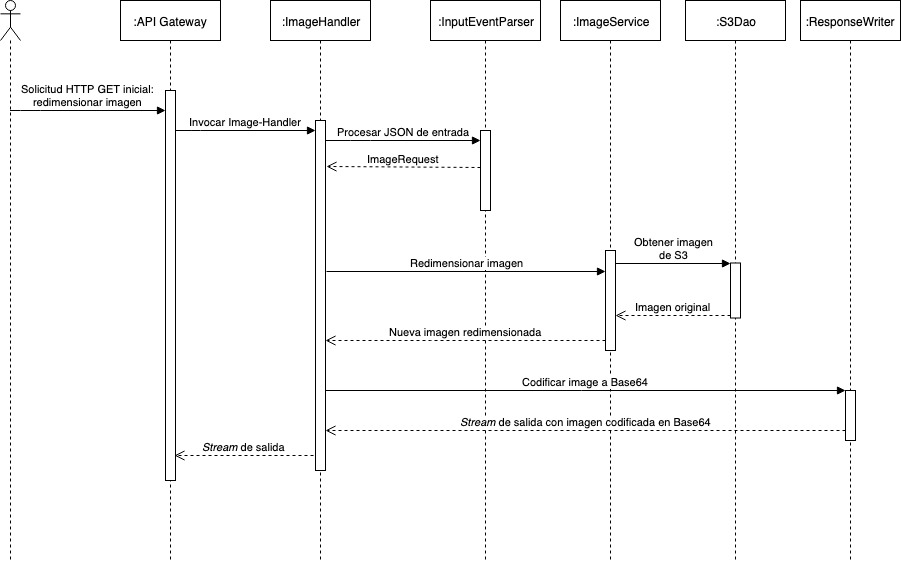
\includegraphics[width=16.5cm]{secuencia-image-handler}
  \caption{Secuencia de acciones llevadas a cabo por \emph{Image-Handler}}
  \label{fig:secuencia-image-handler}
\end{figure}

\subsection{Versiones alternas de \emph{Image-Handler}}

Aparte de la versión original de \emph{Image-Handler}, se crearon dos versiones alternas con el fin de instrumentalizar el código fuente para la extracción y generación de un modelo en PCM a partir, y para la obtención de mediciones del rendimiento. 

En la primer version, el código se modificó para generar rastros del rendimiento de la función Lambda y extraer a partir de estos un modelo de rendimiento en PCM. La segunda versión fue modificada para generar rastros de rendimiento pero, a diferencia de la versión anterior, los datos obtenidos en esta versión fueron de mayor utilidad para afinar las estimaciones de rendimiento de los componentes involucrados en la función.

\subsubsection{Versión instrumentalizada para Kieker y PMX (IM-KP)} \label{sec:image-handler-kieker-pmx}

Uno de los principales objetivos de este trabajo es el de obtener un modelo de rendimiento a partir 
del código en ejecución de una función en la nube. A pesar que, el modelo de rendimiento puede ser creado por los diseñadores e implementadores sin necesidad de una herramienta que ayude a su extracción, el uso de una herramienta especializada para esto contribuye a la generación de un modelo que pueda incluir mayores niveles de detalle en cuanto a la estructura y estimaciones del comportamiento de un software. Además, debido a que se están dando los primeros pasos en el campo del modelado y simulación de rendimiento basado en componentes, es preferible delegar tareas de extracción y estimaciones a una herramienta(s) con el fin de aprender de lo resultados obtenidos e ir introduciendo cambios paulatinamente; la creación manual de modelos de rendimiento puede llegar a ser muy compleja, consumir mucho tiempo y ser propensa a errores. 

Para lograr esto, se seleccionaron dos herramientas, Kieker y PMX, las cuales en conjunto proporcionan un marco de trabajo por medio del cual se puede obtener mediciones del rendimiento de una aplicación y luego, a partir de estas, extraer un modelo de rendimiento basado en PCM. La selección de estas herramientas y el enfoque de medición y extracción de modelos de rendimiento se seleccionó luego de estudiar el \emph{enfoque de ingeniería de rendimiento declarativo} propuesto en \cite{Walter:2018:TDP:3185768.3185777}.


%Kieker se utiliza para el estudiar el comportamiento del rendimiento del sistema a partir de las entradas/rastros que se registran en una bitácora. Creada y mantenida por el grupo de ingeniería de software de la Universidad de Kiel en conjunto con el grupo de sistemas de software de la Universidad de Stuttgart, Kieker se define como una herramienta para monitoreo del rendimiento y análisis dinámico de aplicaciones y se desarolló como parte de las actividades de enseñanza e investigación de ambas universidades. Otras instituciones académicas y de la industria también han realizado contribuciones.

Kieker se utiliza para el estudiar el comportamiento del rendimiento del sistema a partir de las entradas/rastros que se registran en una bitácora. Kieker ofrece adaptadores de monitoreo (\emph{monitoring adapters}) escritos en lenguaje Java (también ofrece adaptadores en otros lenguajes). Los dos principales componentes de Kieker son: \texttt{Kieker.Monitoring} y \texttt{Kieker.Analysis}. \texttt{Kieker.Monitoring} es el responsable de la instrumentación del código, recolección de datos y registro(\emph{logging}). El componente \texttt{Kieker.Analysis} es el responsable de leer, analizar y visualizar los datos monitoreados.

En esta versión de \emph{Image-Handler} se modificó el código original para generar registros del rendimiento de la ejecución de la función utilizando las bibliotecas proporcionadas por Kieker, utilizando como referencia lo especificado en el manual de usuario de Kieker\cite{kieker-user-guide}. Se crean objetos de tipo \texttt{OperationExecutionRecord} los cuales son los que contienen la información acerca del rendimiento de una invocación sobre alguna parte del código.  En el listado \ref{lst:image-handler-kieker} se puede ver un extracto del código de la función instrumentalizada para que genere objetos\\ \texttt{OperationExecutionRecord}.

Adicionalmente se configuró la biblioteca para que publique los objetos\\ \texttt{OperationExecutionRecord} a modo eventos a una cola de mensajería \emph{Java Message Service} (JMS), en lugar de una bitácora local.

\begin{lstlisting}[caption={Extracto de la clase \texttt{ImageHandler.java} instrumentalizada con Kieker}, label={lst:image-handler-kieker}]
public class ImageHandlerKieker implements RequestStreamHandler {
    private static final IMonitoringController MONITORING_CONTROLLER;
    static {
        MONITORING_CONTROLLER = MonitoringController.getInstance();
    }
    .
    .
    .
    
    @Override
    public void handleRequest(InputStream inputStream, OutputStream outputStream, Context context) throws IOException {

        final long tin = MONITORING_CONTROLLER.getTimeSource().getTime();
        handleRequestInternal(inputStream, outputStream, context);
        final long tout = MONITORING_CONTROLLER.getTimeSource().getTime();
        final OperationExecutionRecord e = new OperationExecutionRecord("public void "+ this.getClass().getName()+".handleRequest(InputStream, OutputStream, Context)",
                OperationExecutionRecord.NO_SESSION_ID,
                OperationExecutionRecord.NO_TRACE_ID,
                tin, tout,
                InetAddress.getLocalHost().getHostName(),
                0,
                0);
        MONITORING_CONTROLLER.newMonitoringRecord(e);
    }
    .
    .
    .
}    
\end{lstlisting}


\emph{Performance Model Extractor} (PMX), es una herramienta que automatiza la extracción de modelos de rendmiento a partir de mediciones. PMX utiliza como entrada las bitácoras basadas en Kieker y es capaz de crear modelos basados en \emph{Palladio Component Model} a partir de estas. 

%Esta es una herramienta creada y mantenida por el grupo de ingeniería de software de la Universidad Würzburg en Alemania.

%En conjunto, Kieker y PMX, proporcionan un marco de trabajo por medio del cual se puede obtener mediciones del rendimiento de una aplicación y luego, a partir de estas, extraer un modelo de rendimiento basado en PCM. La selección de estas herramientas y el enfoque de medición y extracción de modelos de rendimiento se seleccionó luego de estudiar el \emph{enfoque de ingeniería de rendimiento declarativo} propuesto en \cite{Walter:2018:TDP:3185768.3185777}.
%
%Esta versión de \emph{Image-Handler} fue la que se utilizó para obtener un modelo de rendimiento en \emph{Palladio Component Model} a partir de la bitácora basada en Kieker que se generó luego de múltiples invocaciones a la función Lambda. El proceso de extracción se detalla en la Sección \ref{sec:estrategia-de-extraccion-de-modelo}.

Los aspectos relacionados con la estrategia de cómo se obtuvo un modelo de rendimiento a partir de las bitácoras de Kieker y PMX se dan a conocer en la Sección \ref{sec:estrategia-de-extraccion-de-modelo}.

\subsubsection{Versión instrumentalizada para AWS X-Ray (IM-XRay)}
La principal motivación detrás de esta nueva versión de \emph{Image-Handler} es la de contar con datos del rendimiento de la función Lambda que no pudieron llegar a ser estimados durante el proceso de extracción del modelo utilizando PMX. En la Sección \ref{sec:estrategia-de-extraccion-de-modelo} se brindan los detalles de lo observado durante el proceso de extracción del modelo con PMX y en dónde encajan los resultados arrojados por esta nueva versión en el modelo.
 
Para esta versión, Se siguió un enfoque similar al de la Sección \ref{sec:image-handler-kieker-pmx} pero en lugar de utilizar la biblioteca de Kieker, se utilizó la biblioteca AWS SDK (\emph{Software Development Kit, SDK}) para crear las trazas y \emph{subsegmentos} de trazas, que son vistas más específicas del comportamiento de la aplicación. Con el uso AWS X-Ray se busca: 
\begin{enumerate}
    \item Obtener datos específicos del rendimiento de la función.
    \item Averiguar si las nuevas mediciones logran brindar información acerca de la infraestructura AWS Lambda y su impacto en la ejecución de \emph{Image-Handler}.
    \item Exportar los datos de rendimiento a algún formato conocido para su manipulación.
\end{enumerate}

Se modificó la función \emph{Image-Handler} para que puede generar trazas de AWS X-Ray en los mismos puntos en el código en los que se agregó la instrumentalización para Kieker. Un extracto de este código se muestra en el listado \ref{lst:image-handler-xray}. Cada invocación a las operaciones de procesamiento de la entrada, redimensionamiento y entrega de la respuesta se realizan utilizando el método \texttt{AWSRay.createSubsegment}.

\begin{lstlisting}[caption={Extracto de la clase \texttt{ImageHandler.java} instrumentalizada con AWS X-Ray}, label={lst:image-handler-xray}]
public class ImageHandlerXRay implements RequestStreamHandler {
    .
    .
    .
    @Override
    public void handleRequest(InputStream inputStream, OutputStream outputStream, Context context) throws IOException {
        ImageRequest imageRequest = AWSXRay.createSubsegment("input event", new Function<Subsegment, ImageRequest>() {
            @Override
            public ImageRequest apply(Subsegment subsegment) {
                return inputEventParser().processInputEvent(inputStream);
            }
        });

        InputStream imageResized = AWSXRay.createSubsegment("resize event", new Function<Subsegment, InputStream>() {
            @Override
            public InputStream apply(Subsegment subsegment) {
                return imageService().getImageFrom(imageRequest);
            }
        });

        AWSXRay.createSubsegment("write response", () -> {
            imageHandlerResponseWriter().writeResponse(imageResized, outputStream, imageRequest);
        });
    }
    .
    .
    .
}
\end{lstlisting}


\begin{figure}[h]
  \centering
  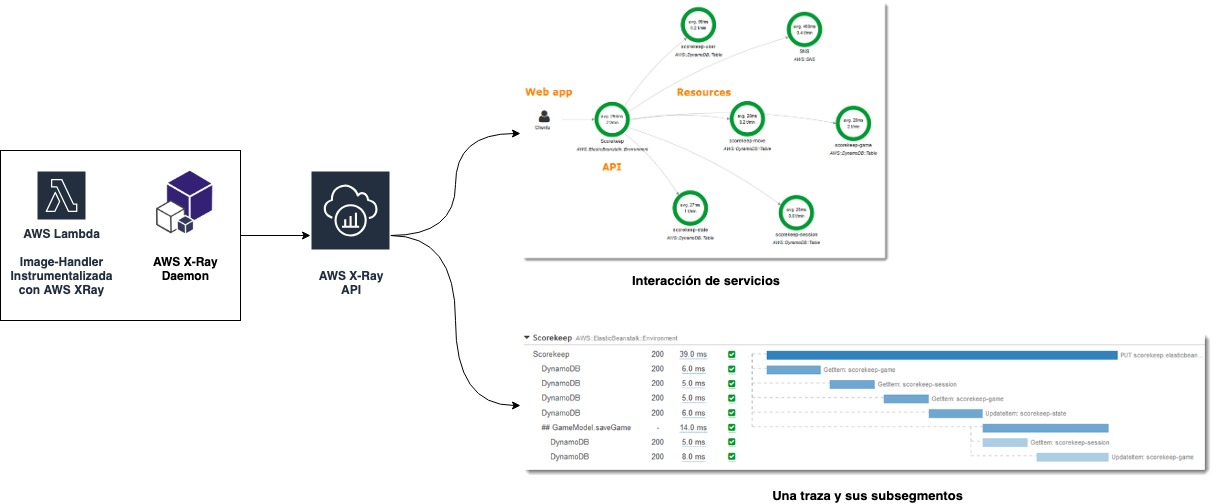
\includegraphics[width=17cm]{image-handler-xray}
  \caption{\emph{Image-Handler} publicando eventos de rendimiento al servicio AWS X-Ray}
  \label{fig:image-handler-xray}
\end{figure}

En la figura \ref{fig:image-handler-xray} se muestran los principales involucrados en la generación de trazas de rendimiento en AWS X-Ray. A la función \emph{Image-Handler} se le agrega la biblioteca de AWS X-Ray para crear las trazas. Estas trazas se envían al servicio AWS X-Ray que es el recolecta estas trazas y con base en ellas se pueden obtener mapas de la interacción de los servicios que componen la función y desgloces de los subsegmentos que componen la traza.


\section{Estrategia de extracción de modelo de rendmiento para \emph{Image-Handler}} \label{sec:estrategia-de-extraccion-de-modelo}
 
Debido a que las funciones Lambda se ejecutan en contenedores que son tanto inaccesibles como efímeros para los diseñadores e implementadores, y, sobre los cuales no se tiene ningún control, estrategias tradicionales en donde se crean bitácoras en la misma computadora en donde se ejecuta la aplicación y se van monitoreando utilizando alguna herramienta especializada o simplemente mediante \emph{Secure Socket Channel}(\texttt{SSH}) deben ser replanteadas. Para este tipo de software, se hace necesario registrar los eventos asociados al comportamiento del rendimiento en una computadora o servicio externo en el cual se tenga control para acceder a los resultados y manipularlos.

Para la extracción del modelo PCM a partir de las bitácoras de Kieker, se llevaron a cabo las siguientes actividades:
\begin{enumerate}
    \item Creación de la versión Image-PK (Sección \ref{sec:image-handler-kieker-pmx}): Versión de \emph{Image-Handler} con las bibliotecas de Kieker para generar bitácoras del rendimiento de la función.    
%    de acuerdo con su manual de usuario\cite{kieker-user-guide}. Se crean objetos de tipo \texttt{OperationExecutionRecord} los cuales contienen información acerca del rendimiento de una invocación sobre alguna parte del código, y luego estos objetos se publican a una cola de mensajería para su posterior tratamiento. En el listado \ref{lst:image-handler-kieker} se puede ver un extracto del código de la función instrumentalizada para que genere objetos  \texttt{OperationExecutionRecord}.
    \item Provisionar una nueva máquina virtual en AWS, en la cual se va a:
    \begin{itemize}
        \item Ejecutar una cola JMS.
        \item Ejecutar una aplicación consumidora de mensajes de la cola JMS.
        \item Almacenar la bitácora de registros de rendimiento de la función Lambda.
    \end{itemize}

    \item Configurar la biblioteca de Kieker para indicar que la publicación de los registros de rendimiento de la función se hagan a través de la cola JMS en la máquina virtual del punto \#2.
    \item Creación de una aplicación consumidora de mensajes para que una vez que arriben los mensajes a la cola JMS, esta procese los mensajes de la cola y los almacene en una bitácora en la máquina virtual creada en el punto \#2. La figura \ref{fig:image-handler-kieker} muestra los involucrados en el proceso de publicación de mediciones de rendimiento del código de \emph{Image-Handler} hacia una bitácora externa.
    \item Una vez obtenida una bitácora en formato Kieker, esta se usó como entrada para PMX. PMX inspecciona la bitácora, la procesa y retorna un archivo \texttt{.zip} con los archivos correspondientes a una instancia de PCM. Lo anterior se aprecia en la figura \ref{fig:image-handler-pmx}.
\end{enumerate}

\subsection{Modelo obtenido}
A partir de la bitácora proporcionada como entrada, PMX logró identificar 6 componentes principales:
\begin{itemize}
    \item \texttt{ImageHandlerKieker}: El punto de entrada de la función.
    \item \texttt{ImageRequestParser}: Encargado de tomar la solicitud de redimensionamiento, analizarla y convertirla en un objeto que pueda ser utilizado por el resto de componentes.
    \item \texttt{S3ImageService}: Contiene la lógica de:
        \begin{enumerate}
            \item Cómo obtener una imagen y
            \item Cómo aplicar la redimiensión sobre la misma.
        \end{enumerate}
    \item \texttt{S3Dao}: El componente que sabe cómo obtener una imagen el servicio AWS S3
    \item \texttt{AmazonS3Client}: Contiene las operaciones de comunicación de bajo nivel con el servicio AWS.
    \item \texttt{HandlerResponseWriter}: Convierte la imagen redimensionada a una representación en \texttt{Base 64} y prepara la respuesta de la función.
\end{itemize}


Cada uno de ellos expone su funcionalidad por medio de una interfaz. En el modelado y simulación basado en componentes, los componentes se conciben como piezas intercambiables los cuales exponen sus operaciones por medio de interfaces y delegan los detalles de implementación a componentes concretos (Como por ejemplo \emph{BasicComponents}). 


Durante las pruebas realizadas al modelo generado por PMX, se percató que si bien el modelo representaba muy bien la intención detrás de los componentes del código fuente, no era detallado en las estimaciones del uso de cada componente. En PCM, a cada componente se le puede especificar su flujo de acciones, estimaciones de rendimiento e invocaciones a otros componentes, por medio de \emph{Service Effect Specifications} (SEFF). 

En principio, las estimaciones incluidas en los SEFFs generados por PMX no lograron ser de utilidad para obtener predicciones representativas de lo observado en las ejecuciones de la función Lambda: mientras que en las invocaciones a \emph{Image-Handler} se entregaban tiempos de respuesta distintos, las simulaciones sobre el modelo entregan siempre un dato fijo. Las estimaciones de rendimiento de los SEFFs se basaban en tiempos de cómputo constantes lo que hacía que el motor de simulaciones generara una predicción del tiempo de respuesta que era el mismo para todos los casos.

%Por esta razón fue se recurrió al trabajo del punto \#3, para obtener datos ``crudos'' del rendimiento de la función Lambda e incluir esto en los \emph{SEFFs} del modelo como distribuciones de frecuencia.



%\begin{lstlisting}[caption={Extracto de la clase \texttt{ImageHandler.java} instrumentalizada con Kieker}, label={lst:image-handler-kieker}]
%public class ImageHandlerKieker implements RequestStreamHandler {
%    private static final IMonitoringController MONITORING_CONTROLLER;
%    static {
%        MONITORING_CONTROLLER = MonitoringController.getInstance();
%    }
%    .
%    .
%    .
%    
%    @Override
%    public void handleRequest(InputStream inputStream, OutputStream outputStream, Context context) throws IOException {
%
%        final long tin = MONITORING_CONTROLLER.getTimeSource().getTime();
%        handleRequestInternal(inputStream, outputStream, context);
%        final long tout = MONITORING_CONTROLLER.getTimeSource().getTime();
%        final OperationExecutionRecord e = new OperationExecutionRecord("public void "+ this.getClass().getName()+".handleRequest(InputStream, OutputStream, Context)",
%                OperationExecutionRecord.NO_SESSION_ID,
%                OperationExecutionRecord.NO_TRACE_ID,
%                tin, tout,
%                InetAddress.getLocalHost().getHostName(),
%                0,
%                0);
%        MONITORING_CONTROLLER.newMonitoringRecord(e);
%    }
%    .
%    .
%    .
%}    
%\end{lstlisting}

% generara registros del rendimiento de la ejecución utilizando las bibliotecas proporcionadas por Kieker, de acuerdo con su manual de usuario\cite{kieker-user-guide}. En lugar de publicar los registros en alguna bitácora local, los registros del rendimiento se publican en una cola \emph{Java Message Service}(JMS). Una vez que arriban los mensajes a la cola JMS, otra aplicación empieza a consumir los mensajes y los va almacenando en una bitácora. 

%La figura \ref{fig:image-handler-kieker} muestra los involucrados en el proceso de publicación de mediciones de rendimiento del código de \emph{Image-Handler} hacia una bitácora externa.

%Una vez que la función Lambda se ejercitó y se haya obtenido una bitácora de Kieker, se toma esta bitácora como entrada para PMX, con el fin de obtener una instancia de PCM. Esto se aprecia en la figura \ref{fig:image-handler-pmx}. Se espera que, al utilizarse datos de mediciones directas del rendimiento de la función Lambda, PMX pueda generar una instacia de PCM que sea confiable y de la que se puedan obtener simulaciones que representativas del comportamiento de la función Lambda.

\begin{figure}[h]
  \centering
  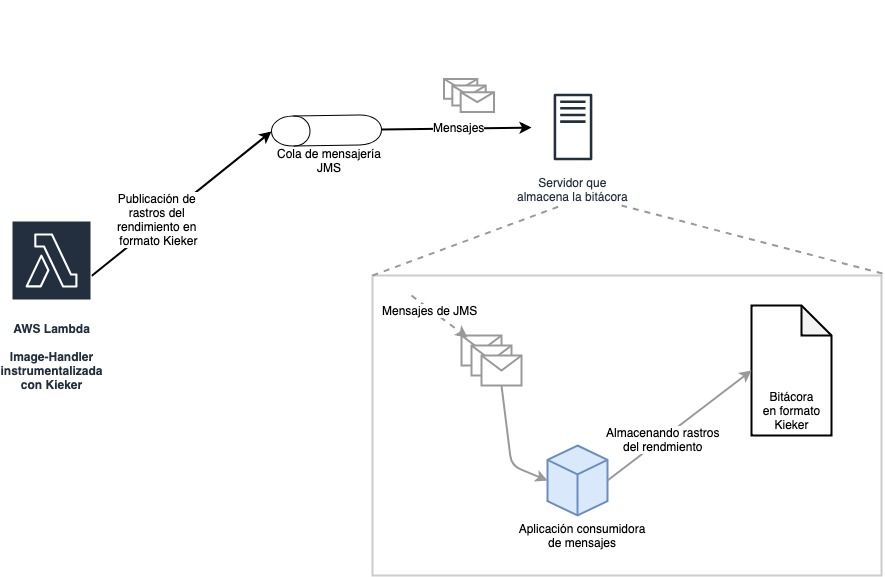
\includegraphics[width=17cm]{image-handler-kieker}
  \caption{Publicando mediciones del rendimiento de la función Lambda.}
  \label{fig:image-handler-kieker}
\end{figure}

\begin{figure}[h]
  \centering
  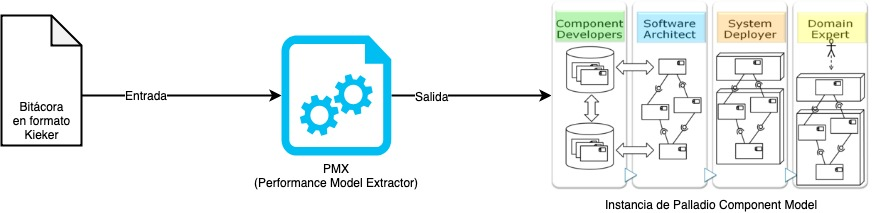
\includegraphics[width=17cm]{image-handler-pmx}
  \caption{Convirtiendo una bitácora de Kieker a una instancia de PCM por medio de PMX.}
  \label{fig:image-handler-pmx}
\end{figure}

\subsubsection{Aporte de la versión IM-XRay a las simulaciones}\label{sec:image-handler-xray}
Una actividad recurrente durante el modelado y simulación de arquitecturas de software, es la del afinamiento del modelo. Esta tarea es necesaria para que el modelo en cual se está trabajando pueda llegar a convertirse una representación cercana del comportamiento de un software en escenarios reales. 

Durante el trabajo con el modelo PCM obtenido en la Sección \ref{sec:image-handler-kieker-pmx} se notó que las estimaciones hechas por PMX no correspondían al comportamiento observado y que el esfuerzo necesario para obtener estas estimaciones a partir de las bitácoras de Kieker podría llegar a ser grande, principalmente porque el formato de las bitácoras de Kieker incluye muchos más datos que solo las estimaciones de rendimiento y porque se empezó a tener la sensación de que estos datos de alguna u otra forma no estaban ``contando toda la historia'' de lo que estaba pasando con la función Lambda. Por ejemplo, las datos de rendimiento de Kieker no podían explicar tiempos de retraso que se observaban al inicio de la ejecución de la función Lambda y, sin esos datos, se podía llegar a generar un modelo poco preciso.

Por esta razón se comenzó a explorar herramientas alternativas para obtener mediciones del rendimiento de la función Lambda y se elegió Amazon X-Ray\footnote{\url{https://aws.amazon.com/xray/}} para este fin. AWS XRay ayuda a los desarrolladores a analizar y depurar aplicaciones en producción distribuidas, tal y como lo son las basadas en arquitecturas de microservicios. Con AWS X-Ray se puede ver cómo es que la aplicación y sus servicios asociados se están ejecutando para identificar y resolver problemas de rendimiento y errores en general.

AWS X-Ray recolecta datos de las solicitudes que hacen a cada uno de los servicios de la aplicación y los agrupa en unas unidades llamadas trazas(\emph{traces}). Luego, utilizando estas trazas, es posible ver mapas de la interacción de los servicios, latencias y metadatos para analizar el comportamiento o identificar problemas.


Las trazas recolectadas en AWS X-Ray fueron de gran utilidad para refinar las estimaciones de rendimiento que cada uno de los componentes identificados realizaba. En el experimento \#1, en la Sección \ref{sec:experimento-1}, se tomaron los datos de rendimiento de cada componente y se realizaron sobre los mismos análisis de frencuencias con el fin de conocer cómo se distribuían estos datos con respecto a sus probabilidades. \textbf{Revisar párrafo con ITZ}. Las probabilidades fueron introducidas en los \emph{SEFFs} de cada componente para la ejecución de simulaciones.   


\section{Diseño Experimental}
En esta sección se detallan los experimentos realizados para:
\begin{itemize}
    \item Validar si el modelo y la simulaciones sobre el mismo, logran caracterizar el comportamiento de la función \emph{Image Handler} en distintos escenarios. 
    \item Estudiar el comportamiento de la función Lambda cuando es invocada con cargas de trabajo y
    \item Comparar los resultados de las invocaciones de la función Lambda con los de la herramienta SAM CLI.
\end{itemize}

\subsection{Utilizando \emph{Image-Handler} para redimensionar imágenes de distintos tamaños} \label{sec:experimento-1}
%Este es el caso que se menciona en la Sección \ref{sec:manejador-imagenes-spe} y se muestra en la figura \ref{fig:serverless-image-handler-architecture-workflow}. Se probó la función Lambda con dos imágines: una de tamaño pequeño ($\sim$100Kb) y otra de tamaño grande ($\sim$5Mb). El objetivo es comprobar cómo los distintos tamaños de las imágenes influyen en el tiempo de respuesta de la función.

Este es el caso que se menciona en la Sección \ref{sec:manejador-imagenes-spe} y se muestra en la figura \ref{fig:serverless-image-handler-architecture-workflow}. Se realizaron invocaciones a la función Lambda con tres grupos de imágenes:
\begin{enumerate}
    \item Imágenes de tamaño menor o igual a 500Kb.
    \item Imágenes de tamaño mayor a 500Kb y menor a 1Mb.
    \item Imágenes de tamaño mayor a 1Mb y menor a 2Mb.
\end{enumerate}
En este experimento, el objetivo es comprobar por medio de mediciones directas y de simulaciones en un modelo, cómo los distintos tamaños de las imágenes influyen en el tiempo de respuesta de la función.

Intuitivamente, se espera que, cuando se hagan solicitudes de redimensionamiento de imágenes de mayor tamaño tomen mayor tiempo en ser procesadas y que lo contrario suceda con las imágenes de menos tamaño. Los resultados obtenidos brindan una referencia inicial para saber cómo es que los componentes de software asociados al redimensionamiento trabajan y qué posibles mejoras podrían realizarse.

Las cargas de trabajo para este experimento son de tipo \emph{cerrada}, lo que quiere decir que una solicitud se ejecuta solamente hasta que la anterior se termina. Esto va orientado a tener mejor trazabilidad de lo que ocurre con la función.

%%%%%%%%%%%%%%%%%%% 1

\subsubsection{Invocaciones con imágenes menores a 500Kb}
Para la realización de este experimento se contó con la siguiente configuración base:
\begin{itemize}
    \item \emph{Sujeto de prueba:} La función Lambda IM-Simple.
    \item \emph{Repositorio de imágenes:} \emph{Cluster} de 1000 imágenes de tamaño menor a 500Kb alojadas en Amazon S3.     
    \item \emph{Carga de trabajo:} 1000 invocaciones secuenciales de redimensionamiento de imágenes con dimensiones aleatorias a IM-Simple.
    \item \emph{Herramientas de medición:} Amazon Cloudwatch.
\end{itemize}

Configuración para la obtención de datos de rendimiento

\begin{itemize}
    \item \emph{Sujeto de prueba:} Las funciones Lambda IM-KP y IM-XRay
    \item \emph{Repositorio de imágenes:} \emph{Cluster} de 1000 imágenes de tamaño menor a 500Kb alojadas en Amazon S3.     
    \item \emph{Carga de trabajo:} 1000 invocaciones secuenciales de redimensionamiento de imágenes con dimensiones aleatorias a IM-PK y IM-XRay.
    \item \emph{Herramientas de medición:} Kieker, PMX y Amazon X-Ray.
\end{itemize}

Para la realización de este experimento, se obtuvieron 1000 imágenes aleatorias de tamaño menor a 500Kb del servicio \emph{Lorem Picsum}\footnote{\url{https://picsum.photos}}. Se creó un \emph{script} en \texttt{Bash} para acceder a la interfaz de programación (API) proporcionada por \emph{Lorem Picsum} para descargar de forma aleatoria 1000 imágenes cuyo tamaño era menor a los 500Kb. La distribución del tamaño de las 1000 imágenes, en Kb, se aprecia en la figura \ref{fig:distribucion-tamanno-imagenes-hasta-500kb}. El mismo grupo de imágenes se utilizó para realizar solicitudes de redimensionamiento sobre IM-Simple, IM-KP y IM-XRay.

\begin{figure}
\hspace{-1cm}
\begin{tikzpicture}
\begin{axis}[
  width=15cm, height=10cm,
  title={\textbf{Distribución del tamaño de imágenes de tamaño $\leq 500Kb$}},
  ylabel={\small Cantidad de imágenes},
  x label style={at={(axis description cs:0.5,-0.1)},anchor=north},
  xlabel={\small Tamaño de las imágenes (En $Kb$)},
  xmin=0, ymin=0, xmax=550,
  ybar interval,
  xtick=data,
  xticklabel interval boundaries,
  x tick label style={rotate=30,anchor=east}
  ],
	\addplot+[hist={bins=10}]
		table[col sep=comma, y index=0] {datos/tamannos-cluster-a.csv};
\end{axis}
\end{tikzpicture}
\caption{Distribución del tamaño de imágenes $\leq 500Kb$}
\label{fig:distribucion-tamanno-imagenes-hasta-500kb}
\end{figure}

\paragraph{Medición Base: 1000 invocaciones de redimensionamiento de imágenes en IM-Simple.} 
Se creó un \emph{script} en \texttt{Bash} para ejecutar 1000 invocaciones de redimensionamiento en la función IM-Simple en las imágenes de tamaño menor a 500Kb. El \emph{script} selecciona una imagen de forma aleatoria y luego ejecuta la solicitud de redimensionamiento utilizando dimensiones de ancho y alto de uso común para imágenes en miniatura (\emph{thumbnails}) \textbf{AGREGAR APARTADO SOBRE LA ELECCION LOS THUMBNAILS}.

\begin{figure}[h]
\hspace{-1.0cm}
\begin{tikzpicture}
\begin{axis}[
  width=16cm, height=8cm,
  title style={align=center},
  title={\textbf{Distribución de los tiempos de respuesta en solicitudes de redimensionamiento}\\\textbf{de imágenes de tamaño $\leq 500Kb$ en IM-Simple}},
  ylabel={\small Solicitudes de redimensionamiento},
  x label style={at={(axis description cs:0.5,-0.21)},anchor=north},
  xlabel={\small Tiempos de respuesta (En $ms$)},
  xmin=0, ymin=0, xmax=4020,
  ybar interval,
  xtick=data,
  xticklabel interval boundaries,
  x tick label style={rotate=30,anchor=east}
  ],
	\addplot+[fill=red!70!white,hist={bins=10}]
		table[col sep=comma, y index=0] {datos/tiempos-de-respuesta-hasta-500kb-simple.csv};
\end{axis}
\end{tikzpicture}
\caption{Distribución de los tiempos de respuesta en solicitudes de redimensionamiento de imágenes de tamaño $\leq 500Kb$ en IM-Simple}
\label{fig:distribucion-solicitudes-imagenes-hasta-500kb}
\end{figure}

\begin{figure}[h]
%\vspace{-4cm}
\hspace{-1.0cm}
\begin{tikzpicture}
\begin{axis}[
  width=16cm, height=8cm,
  title style={align=center},
  title={\textbf{Distribución de los tiempos de respuesta en solicitudes de redimensionamiento}\\\textbf{de imágenes de tamaño $\leq 500Kb$ en las simulaciones de Palladio}},
  ylabel={\small Solicitudes de redimensionamiento},
  xmin=0, ymin=0, xmax=4000,
  ybar interval,
  xtick=data,
  x label style={at={(axis description cs:0.5,-0.2)},anchor=north},
  xlabel={\small Tiempos de respuesta (En $ms$)},  
  xticklabel interval boundaries,
  x tick label style={rotate=30,anchor=east}
  ],
	\addplot+[hist={bins=10}]
		table[col sep=comma, y index=0] {datos/tiempos-de-respuesta-hasta-500kb-palladio.csv};
\end{axis}
\end{tikzpicture}
\caption{Distribución de los tiempos de respuesta en solicitudes de redimensionamiento de imágenes de tamaño $\leq 500Kb$ en las simulaciones de \emph{Palladio Workbench}}
\label{fig:distribucion-simulacion-imagenes-hasta-500kb}
\end{figure}

En la figura \ref{fig:distribucion-solicitudes-imagenes-hasta-500kb} se muestra la distribución de los tiempos de respuesta en las solicitudes de redimensionamiento en las imágenes de tamaño menor a 500Kb. Con excepción de la primera invocación, la cual tuvo una duración de 4 segundos, más del 97,5\% de las invocaciones no superó los 1,6 segundos.

\paragraph{Mediciones para obtención de modelo de rendimiento: 1000 invocaciones de redimensionamiento de imágenes en IM-PK y IM-XRay.} Se utilizó el mismo \emph{script} en \texttt{Bash} y la misma configuración para generar invocaciones a la función Lambda descrita en la sección anterior.

En primera instancia se ejecutaron 1000 invocaciones a IM-PK para generar una bitácora de Kieker y a partir de la misma extraer un modelo de rendimiento PCM usando PMX. Tal y como se señala en la Sección \ref{sec:image-handler-xray}, las estimaciones hechas por PMX sobre el rendimiento de los componentes del modelo se basaban en valores constantes. Fue por esta razón que, para contar con una versión alternativa de \emph{Image Handler} que pudiera brindar otro nivel de detalle en las  métricas de rendimiento, se introdujo IM-XRay.

Al igual que en caso anterior, se ejecutaron 1000 invocaciones a IM-XRay, y por medio de un \emph{script} en \texttt{Bash}, se obtuvieron las trazas correspondientes a las 1000 invocaciones. Los nuevos datos fueron exportados a formato \texttt{.csv} e interpretados con el lenguaje \texttt{R}. En \texttt{R}, se calcularon distribuciones de frecuencia de la probabilidad en la que un componente lograba procesar una porción de la carga de trabajo total. Estos datos fueron incluidos en los \emph{SEEFs} de cada componente del modelo. Por último se ejecutó una simulación en \emph{Palladio Workbench} con los siguientes parámetros:
\begin{itemize}
    \item Generación de 1000 mediciones.
    \item Carga de trabajo: \emph{cerrada}. Se ejecuta una solicitud sobre el modelo hasta que la anterior termina. 
\end{itemize}

%\hspace{-4cm}
\begin{table}
    \centering
    \begin{tabular}{l|r|r|r}
        \toprule[1.5pt]
        \multicolumn{4}{c}{\textbf{Hasta 500Kb}} \\
        \midrule
        Solicitud de redimensionamiento  & IM-Simple & PCM & Diferencia\\
        \midrule
        Tiempo promedio  & 583.842ms & 793.808ms & 209.965ms\\
        Desviación estándar & 460.659ms & 465.441ms & 4.782ms\\
        Varianza & 212206.961 & 216635 & -- \\
        Mediana & 466.715ms & 680.482ms &. -- \\
        Coeficiente de variación & 0.987 & 0.683 & -- \\                       
        \bottomrule[1.5pt]
    \end{tabular}
    \caption{Resumen de datos estadísticos}
    \label{table:datos-estadisticos-hasta-500kb}
\end{table}

En la figura \ref{fig:distribucion-simulacion-imagenes-hasta-500kb}, se muestra la distribución de los tiempos de respuesta en las solicitudes de redimensionamiento en las simulaciones de \emph{Palladio Workbench} para imágenes de tamaño $\leq 500Kb$. En los resultados de las simulaciones, el 95\% de las invocaciones no superó los 1,6 segundos en procesar la solicitud de redimensionamiento.

En este punto, se cuenta con 1000 mediciones hechas sobre IM-Simple y un modelo al que se le simularon 1000 invocaciones. En la figura \ref{fig:comparacion-imsimple-palladio-500kb} se comparan los tiempos de respuesta obtenidos en IM-Simple y los de las simulaciones, y, en el Cuadro \ref{table:datos-estadisticos-hasta-500kb}, un resumen de los datos estadísticos de los tiempos de respuesta en ambos sujetos de prueba.

\begin{figure}[h]
\hspace{-1cm}
\begin{tikzpicture}
	\begin{axis}[
	width=16cm, height=12cm, xmin=0, ymin=0,
	xmax=1010, ymax=4500,
	title={\textbf{1000 Solicitudes de redimensionamiento de imágenes de tamaño $\leq 500Kb$}},
	xlabel={\small Número de ejecución de solicitud de redimensionamiento},
	ylabel={\small Milisegundos},
	grid=major, grid style=dashed, label style={font=\small},
%	extra y ticks={400,600},
%	extra y tick labels={PP, PIM},
   extra y tick style={%
     color=green,
    },	
	tick label style={font=\footnotesize},
	scatter/classes={%
		a={mark=square*,blue},%
		b={mark=square*,red},%
		c={mark=o,draw=black}}]					
	\addplot[scatter,only marks,%
		scatter src=explicit symbolic]%
	table[meta=label, col sep=comma] {datos/xy-data-hasta-500kb.csv};
	
	\legend{Simulaciones de Palladio, Solicitudes a IM-Simple}
	\end{axis}
\end{tikzpicture}
\caption{IM-Simple \emph{vs} simulaciones en PCM: 1000 solicitudes de redimensionamiento de imágenes de tamaño $\leq 500Kb$.}
\label{fig:comparacion-imsimple-palladio-500kb}
\end{figure}

\begin{figure}[h]
\hspace{-1.5cm}
\begin{tikzpicture}
\begin{axis}[
    width=16cm, height=12cm,
    title={\small \textbf{Probabilidad acumulada: solicitudes de redimensionamiento en imágenes $\leq 500Kb$ en PCM}},
    xlabel={\small Segundos},
    ylabel={\small Probabilidad acumulada},
    xmin=0, xmax=4.2,
    ymin=0, ymax=1.05,
    extra y ticks = {0.9,0.95},
    extra x tick style={tick label style={font=\footnotesize}},    
	legend style={at={(0.5,-0.15)},
		anchor=north,legend columns=-1},
    grid=major,
    grid style=dashed,
]

\addplot[mark=none,blue,smooth] table [col sep=comma] {datos/hasta-500kb-cdf.csv};

\coordinate (a) at (axis cs:1.6, 0.95);
\draw[blue, dashed, thick](a |- current plot begin) -- (a);
 
\end{axis}
\end{tikzpicture}
\caption{Probabilidad acumulada en solicitudes de redimensionamiento en imágenes de tamaño $\leq 500Kb$ en \emph{Palladio Workbench}}
\label{fig:funcion-acumulada-palladio-500kb}
\end{figure}

\subsubsection{Análisis de resultados} 
La Figura \ref{fig:comparacion-imsimple-palladio-500kb} muestra un panorama alentador. Las ejecuciones de las simulaciones en PCM presentan tiempos de respuesta muy similares a los que entrega IM-Simple. Hay una diferencia de 209,965ms en el tiempo promedio de los tiempos de respuesta de las simulaciones en PCM con respecto a los tiempos de IM-Simple. Preliminarmente, se valora que, debido a que la versión IM-XRay tiene activado el servicio de monitoreo AWS X-Ray y que fue esta versión de \emph{Image Handler} utilizada como referencia para generar los tiempos procesamiento estimados para cada componente del modelo, instrumentalizar la función Lambda con el servicio de monitoreo AWS X-Ray genera un \emph{overhead} en el procesamiento de la función. Cabe mencionar que, la estrategia de monitoreo utilizada fue muy agresiva debido a que para obtener nuevas métricas para los componentes del modelo PCM, se habilitaron muchos puntos de monitoreo dentro del código fuente. Además, se configuró la función Lambda para que monitoreara el 100\% de las invocaciones a solicitudes de redimensionamiento. Esta configuración de monitoreo no es la habitual que se utiliza para las funciones Lambda en producción, pero, para el caso de este estudio se necesitó contar con mayores niveles de detalle en las mediciones por lo que fue necesario sacar el mayor provecho al monitoreo. Entre menor sea utilizado las opciones de monitoreo de AWS X-Ray en la función Lambda, menor será el \emph{overhead} experimentado, tal y como pasa con IM-Simple en donde no se experiementa \emph{overhead} por concepto de monitoreo.

Los resultados muestran desviaciones estándar de 460,569ms y 465.445ms para IM-Simple y las simulaciones de PCM respectivamente. La desviación estándar de las simulaciones de PCM es solamente 4,782ms mayor que la de IM-Simple, lo que sugiere que la agrupación de los datos con respecto a su media aritmética serán muy semejantes.

Los coeficientes de variación para IM-Simple y las simulaciones de PCM fue de 0.987 y 0.683 respectivamente. Estos resultados, apuntan a una mayor heterogeneidad entre los tiempos de respuesta y a que el tiempo promedio de procesamiento no se considere representativo para este conjunto de datos. Esta variabilidad viene dada por las diferencias de los tamaños de las imágenes utilizadas para este experimento, como se muestra en la Figura \ref{fig:distribucion-tamanno-imagenes-hasta-500kb}: imágenes de tamaño $\leq 500Kb$, en donde existen diferencias de hasta 500x, por lo que, por ejemplo, el tiempo de procesamiento de una imagen de tamaño de 5kb será más rápido que una de tamaño de 490Kb.

Por último, de acuerdo con los resultados de las simulaciones, existe un 95\% de probabilidad de que el tiempo de procesamiento de una solicitud de redimensionamiento de una imagen de tamaño $\leq 500Kb$ tome 1,6 segundos o menos (Figura \ref{fig:funcion-acumulada-palladio-500kb}). En IM-Simple, se obtuvo un 97,5\% de probabilidad para el mismo caso (Figura \ref{fig:distribucion-solicitudes-imagenes-hasta-500kb}). Para este caso en particular y, debido a la variabilidad de los tiempos de respuesta, se considera que el uso de esta probabilidad acumulada es más representativa a la hora de describir el comportamiento de la función Lambda.

%%%%%%%%%%%%%%%%%%% 2

\subsubsection{Invocaciones con imágenes mayores a 500Kb y menores o igual a 1Mb}
Para la realización de este experimento se contó con la siguiente configuración base:
\begin{itemize}
    \item \emph{Sujeto de prueba:} La función Lambda IM-Simple.
    \item \emph{Repositorio de imágenes:} \emph{Cluster} de 1000 imágenes de tamaño mayor a 500Kb y menor o igual a 1Mb alojadas en Amazon S3.     
    \item \emph{Carga de trabajo:} 1000 invocaciones secuenciales de redimensionamiento de imágenes con dimensiones aleatorias a IM-Simple.
    \item \emph{Herramientas de medición:} Amazon Cloudwatch.
\end{itemize}

Configuración para la obtención de datos de rendimiento

\begin{itemize}
    \item \emph{Sujeto de prueba:} La función IM-XRay
    \item \emph{Repositorio de imágenes:} \emph{Cluster} de 1000 imágenes de tamaño mayor a 500Kb y menor o igual a 1Mb alojadas en Amazon S3.     
    \item \emph{Carga de trabajo:} 1000 invocaciones secuenciales de redimensionamiento de imágenes con dimensiones aleatorias a IM-XRay.
    \item \emph{Herramientas de medición:} Amazon X-Ray.
\end{itemize}

Para este experimento no realizó ningún trabajo sobre la versión IM-KP porque no se necesita extraer ningún modelo. El modelo fue extraído y generado en el experimento anterior y debido a que se usa es el mismo código con los mismos puntos de monitoreo, un eventual proceso de extracción daría como resultado el mismo modelo del experimento anterior. Lo que sí fue necesario hacer, fue calibrar el modelo existente con los resultados de las mediciones a solicitudes de redimensionamiento en imágenes de tamaño mayor a 500Kb y menor o igual 1Mb, utilizando la versión IM-XRay. 

Para la realización de este experimento, se obtuvieron 1000 imágenes aleatorias de tamaño mayor a 500Kb y menor o igual a 1Mb del servicio \emph{Lorem Picsum}. Se ejecutó el \emph{script} en \texttt{Bash} del experimento anterior para acceder a la API de \emph{Lorem Picsum} para descargar de forma aleatoria 1000 imágenes cuyo tamaño fuera mayor a los 500Kb y menor o igual a 1Mb. La distribución del tamaño de las 1000 imágenes, en Kb, se aprecia en la figura \ref{fig:distribucion-tamanno-imagenes-hasta-1mb}. El mismo grupo de imágenes se utilizó para realizar solicitudes de redimensionamiento sobre IM-Simple y IM-XRay.

\begin{figure}
\hspace{-1.0cm}
\begin{tikzpicture}
\begin{axis}[
  width=15cm, height=10cm,
  title={\textbf{Distribución del tamaño de imágenes de tamaño $500Kb \leq x \leq 1Mb$}},
  ylabel={\small Cantidad de imágenes},
  x label style={at={(axis description cs:0.5,-0.2)},anchor=north},
  xlabel={\small Tamaño de las imágenes (En $Kb$)},
  xmin=0, ymin=0, xmin=500, xmax=1024,
  ybar interval,
  xtick=data,
  xticklabel interval boundaries,
  x tick label style={rotate=45,anchor=east}  
  ],
	\addplot+[hist={bins=10}]
		table[col sep=comma, y index=0] {datos/tamannos-cluster-b.csv};
\end{axis}
\end{tikzpicture}
\caption{Distribución del tamaño de imágenes $500Kb \leq x \leq 1Mb$}
\label{fig:distribucion-tamanno-imagenes-hasta-1mb}
\end{figure}

\paragraph{Medición Base: 1000 invocaciones de redimensionamiento de imágenes en IM-Simple.} 
Se ejecutó el \emph{script} en \texttt{Bash} del experimento anterior para ejecutar 1000 invocaciones de redimensionamiento en la función IM-Simple en las imágenes de tamaño mayor a 500Kb y menor o igual a 1Mb. El \emph{script} selecciona una imagen de forma aleatoria y luego ejecuta la solicitud de redimensionamiento utilizando dimensiones de ancho y alto de uso común para imágenes en miniatura.

\begin{figure}
\hspace{-1.0cm}
\begin{tikzpicture}
\begin{axis}[
  width=16cm, height=8cm,
  title style={align=center},
  title={\textbf{Distribución de los tiempos de respuesta en solicitudes de redimensionamiento}\\\textbf{de imágenes de tamaño $500Kb \leq x \leq 1Mb$ en IM-Simple}},
  ylabel={\small Solicitudes de redimensionamiento},
  x label style={at={(axis description cs:0.5,-0.21)},anchor=north},
  xlabel={\small Tiempos de respuesta (En $ms$)},
  xmin=0, ymin=0, xmax=8500,
  ybar interval,
  xtick=data,
  xticklabel interval boundaries,
  x tick label style={rotate=30,anchor=east}
  ],
	\addplot+[fill=red!70!white,hist={bins=10}]
		table[col sep=comma, y index=0] {datos/tiempos-de-respuesta-hasta-1mb-simple.csv};
\end{axis}
\end{tikzpicture}
\caption{Distribución de los tiempos de respuesta en solicitudes de redimensionamiento de imágenes de tamaño $500Kb \leq x \leq 1Mb$ en IM-Simple}
\label{fig:distribucion-solicitudes-imagenes-hasta-1mb}
\end{figure}


En la figura \ref{fig:distribucion-solicitudes-imagenes-hasta-1mb} se muestra la distribución de los tiempos de respuesta en las solicitudes de redimensionamiento en las imágenes de tamaño mayor a 500Kb y menor o igual a 1Mb. Más del 98\% de las invocaciones no superó los 8 segundos.

\paragraph{Mediciones para la calibración de modelo de rendimiento: 1000 invocaciones de redimensionamiento de imágenes en IM-XRay.} Se utilizó el mismo \emph{script} en \texttt{Bash} y la misma configuración para generar invocaciones a la función Lambda descrita en la sección anterior.

Se ejecutaron 1000 invocaciones a IM-XRay, y por medio de un \emph{script} en \texttt{Bash}, se obtuvieron las trazas correspondientes a las 1000 invocaciones. Los nuevos datos fueron exportados a formato \texttt{.csv} e interpretados con el lenguaje \texttt{R}. En \texttt{R}, se calcularon distribuciones de frecuencia de la probabilidad en la que un componente lograba procesar una porción de la carga de trabajo total. Estos datos fueron incluidos en los \emph{SEEFs} de cada componente del modelo. Por último se ejecutó una simulación en \emph{Palladio Workbench} con los siguientes parámetros:
\begin{itemize}
    \item Generación de 1000 mediciones.
    \item Carga de trabajo: \emph{cerrada}. Se ejecuta una solicitud sobre el modelo hasta que la anterior termina. 
\end{itemize}

\hspace{-2.0cm}
\begin{figure}
\begin{tikzpicture}
\begin{axis}[
  width=16cm, height=8cm,
  title style={align=center},
  title={\textbf{Distribución de los tiempos de respuesta en solicitudes de redimensionamiento}\\\textbf{de imágenes de tamaño $500Kb \leq x \leq 1Mb$ en las simulaciones de Palladio}},
  ylabel={\small Solicitudes de redimensionamiento},
  x label style={at={(axis description cs:0.5,-0.21)},anchor=north},
  xlabel={\small Tiempos de respuesta (En $ms$)},  
  xmin=0, ymin=0, xmax=9300,
  ybar interval,
  xtick=data,
  xticklabel interval boundaries,
  x tick label style={rotate=30,anchor=east}
  ],
	\addplot+[hist={bins=10}]
		table[col sep=comma, y index=0] {datos/tiempos-de-respuesta-hasta-1mb-palladio.csv};
\end{axis}
\end{tikzpicture}
\caption{Distribución de los tiempos de respuesta en solicitudes de redimensionamiento de imágenes de tamaño $500Kb \leq x \leq 1Mb$ en las simulaciones de Palladio}
\label{fig:distribucion-simulacion-imagenes-hasta-1mb}
\end{figure}

En la figura \ref{fig:distribucion-simulacion-imagenes-hasta-1mb}, se muestra la distribución de los tiempos de respuesta en las solicitudes de redimensionamiento en las simulaciones de \emph{Palladio Workbench} para imágenes de tamaño mayor a 500Kb y menor o igual a 1Mb. En los resultados de las simulaciones, el 95\% de las invocaciones no superó los 8 segundos en procesar la solicitud de redimensionamiento.

En este punto, se cuenta con 1000 mediciones hechas sobre IM-Simple y un modelo al que se le simularon 1000 invocaciones. En la figura \ref{fig:comparacion-imsimple-palladio-1mb} se comparan los tiempos de respuesta obtenidos en IM-Simple y los de las simulaciones, y, en el Cuadro \ref{table:datos-estadisticos-hasta-1mb}, un resumen de los datos estadísticos de los tiempos de respuesta en ambos sujetos de prueba.

\begin{figure}[h]
\hspace{-1cm}
\begin{tikzpicture}
	\begin{axis}[
	width=16cm, height=12cm, xmin=0, ymin=0,
	xmax=1010, 
	ymax=9500,
	title={\textbf{Solicitudes de redimensionamiento de imágenes de tamaño $500Kb \leq x \leq 1Mb$}},
	xlabel={Número de ejecución de solicitud de redimensionamiento},
	ylabel={Milisegundos},
	grid=major, grid style=dashed, label style={font=\small},
	tick label style={font=\footnotesize},
	scatter/classes={%
		a={mark=square*,blue},%
		b={mark=square*,red},%
		c={mark=o,draw=black}}]			
	\addplot[scatter,only marks,%
		scatter src=explicit symbolic]%
	table[meta=label, col sep=comma] {datos/xy-data-hasta-1mb.csv};
	\legend{Simulaciones de Palladio, Solicitudes a \emph{Image Handler}}
	\end{axis}
\end{tikzpicture}
\caption{Solicitudes de redimensionamiento de imágenes de tamaño $500Kb \leq x \leq 1Mb$}
\label{fig:comparacion-imsimple-palladio-1mb}
\end{figure}

\begin{table}
    \centering
    \begin{tabular}{l|r|r|r}
        \toprule[1.5pt]
         \multicolumn{4}{c}{\textbf{Entre 500Kb a 1Mb}} \\
        \midrule
        Solicitud de redimensionamiento  & Image Handler & Palladio & Diferencia\\  
        \midrule        
        Tiempo promedio  & 4073.600ms & 4348.029ms & 274.428ms\\
        Desviación estándar & 1731.974ms & 1844.893ms & 112.919ms\\
        Varianza & 2999736.844 & 3403633.84 & --\\
        Mediana & 3658.825ms & 3989.406ms & -- \\
        Coeficiente de variación & 0.473 & 0.462 & -- \\                      
        \bottomrule[1.5pt]
    \end{tabular}
    \caption{Resumen de datos estadísticos}
    \label{table:datos-estadisticos-hasta-1mb}
\end{table}

\subsubsection{Análisis de resultados}
A primera vista, la comparación de los tiempos de respuesta de IM-Simple y las simulaciones en PCM mostradas en la Figura \ref{fig:comparacion-imsimple-palladio-1mb} muestran gran similitud. Hay una diferencia de 274,428ms en el tiempo promedio de los tiempos de respuesta en las simulaciones PCM con respecto a los tiempos de IM-Simple. En este experimento también se intuye que la estrategia de monitoreo de AWS X-Ray es la resposable de agregar este \emph{overhead} en el procesamiento.

Los resultados muestran desviaciones estándar de 1731.974ms y 1844.893ms para IM-Simple y las simulaciones de PCM respectivamente. La desviación estándar de las simulaciones de PCM es 112.919ms mayor que la de IM-Simple. Esto indica que la agrupación de los datos con respecto a su media aritmética es muy similar entre ambas muestras.

Los coeficientes de variación de ambas muestras bajaron con respecto a los obtenidos en el primer experimento, aún así, los valores de 0,473 para IM-Simple y de 0,462 para las simulaciones de PCM se consideran heterogéneos, no muy similares entre si. Esto hace que el tiempo promedio de una solicitud pueda considerarse no tan representativo a la hora de caracterizar el comportamiento de la función Lambda bajo esta carga de trabajo. La variabilidad en los tiempos de respuesta bajó debido a que en los tamaños de las imágenes utilizadas (Figura \ref{fig:distribucion-tamanno-imagenes-hasta-1mb}) tienen una diferencia de hasta 2 veces: es decir, en este conjunto, la imagen más grande es el doble de grande que la imagen más pequeña.

Por último, de acuerdo con los resultados de las simulaciones, existe un 95\% de probabilidad de que el tiempo de procesamiento de una solicitud de redimensionamiento de una imagen de tamaño $500Kb \leq x \leq 1Mb$ tome 8 segundos o menos (Figura \ref{fig:funcion-acumulada-palladio-1mb}). En IM-Simple, se obtuvo un 98\% de probabilidad para el mismo caso (Figura \ref{fig:distribucion-solicitudes-imagenes-hasta-1mb}). Para este caso, como en el experimento anterior, se considera más adecuado el uso de la probabilidad acumulada para describir el comportamiento de la función Lambda.

\begin{figure}
\hspace{-2cm}
\begin{tikzpicture}
\begin{axis}[
    width=16cm, height=12cm,
    title={\small \textbf{Probabilidad acumulada: solicitudes de redimensionamiento en imágenes $500Kb \leq x \leq 1Mb$ en PCM}},
    xlabel={\small Segundos},
    ylabel={\small Probabilidad acumulada},
    xmin=0, xmax=10,
    ymin=0, ymax=1.05,
    extra y ticks = {0.9,0.95},
    extra x tick style={tick label style={font=\footnotesize}},    
	legend style={at={(0.5,-0.15)},
		anchor=north,legend columns=-1},
    grid=major,
    grid style=dashed,
]
\addplot[mark=none,blue,smooth] table [col sep=comma] {datos/hasta-1mb-cdf.csv};
\coordinate (b) at (axis cs:8.0, 0.95);
\draw[blue, dashed, thick](b |- current plot begin) -- (b);
\end{axis}
\end{tikzpicture}
\caption{Probabilidad acumulada de solicitudes de redimensionamiento en imágenes $500Kb \leq x \leq 1Mb$ en PCM}
\label{fig:funcion-acumulada-palladio-1mb}
\end{figure}

%%%%%%%%%%%%%%%%%%% 3

\subsubsection{Invocaciones con imágenes mayores a 1Mb y menores o igual a 2Mb}
Para la realización de este experimento se contó con la siguiente configuración base:
\begin{itemize}
    \item \emph{Sujeto de prueba:} La función Lambda IM-Simple.
    \item \emph{Repositorio de imágenes:} \emph{Cluster} de 1000 imágenes de tamaño mayor a 1Mb y menor o igual a 2Mb alojadas en Amazon S3.     
    \item \emph{Carga de trabajo:} 1000 invocaciones secuenciales de redimensionamiento de imágenes con dimensiones aleatorias a IM-Simple.
    \item \emph{Herramientas de medición:} Amazon Cloudwatch.
\end{itemize}

Configuración para la obtención de datos de rendimiento

\begin{itemize}
    \item \emph{Sujeto de prueba:} La función IM-XRay
    \item \emph{Repositorio de imágenes:} \emph{Cluster} de 1000 imágenes de tamaño mayor a 1Mb y menor o igual a 2mb alojadas en Amazon S3.     
    \item \emph{Carga de trabajo:} 1000 invocaciones secuenciales de redimensionamiento de imágenes con dimensiones aleatorias a IM-XRay.
    \item \emph{Herramientas de medición:} Amazon X-Ray.
\end{itemize}

Al igual que en el experimento de la sección anterior, no se realizó ningún trabajo sobre la versión IM-KP debido a que no era necesario la extracción de un nuevo modelo, sino de, calibrar el modelo existente con los resultados de las mediciones para generar nuevas simulaciones.

Para la realización de este experimento, se obtuvieron 1000 imágenes aleatorias de tamaño mayor a 1Mb y menor o igual a 2Mb del servicio \emph{Lorem Picsum}. Se ejecutó el \emph{script} en \texttt{Bash} del experimento anterior para acceder a la API de \emph{Lorem Picsum} para descargar de forma aleatoria 1000 imágenes cuyo tamaño fuera mayor a 1Mb y menor o igual a 2Mb. La distribución del tamaño de las 1000 imágenes, en Kb, se aprecia en la figura \ref{fig:distribucion-tamanno-imagenes-hasta-2mb}. El mismo grupo de imágenes se utilizó para realizar solicitudes de redimensionamiento sobre IM-Simple y IM-XRay.

\begin{figure}
\hspace{-1.0cm}
\begin{tikzpicture}
\begin{axis}[
  width=15cm, height=10cm,
  title={\textbf{Distribución del tamaño de imágenes de tamaño $1Mb \leq x \leq 2Mb$}},
  ylabel={\small Cantidad de imágenes},
  x label style={at={(axis description cs:0.5,-0.2)},anchor=north},
  xlabel={\small Tamaño de las imágenes (En $Kb$)},  
  xmin=0, ymin=0, xmin=1000, xmax=2048,
  ybar interval,
  xtick=data,
  xticklabel interval boundaries,
  x tick label style={rotate=30,anchor=east}  
  ],
	\addplot+[hist={bins=10}]
		table[col sep=comma, y index=0] {datos/tamannos-cluster-c.csv};
\end{axis}
\end{tikzpicture}
\caption{Distribución del tamaño de imágenes de tamaño $1Mb \leq x \leq 2Mb$}
\label{fig:distribucion-tamanno-imagenes-hasta-2mb}
\end{figure}

\paragraph{Medición Base: 1000 invocaciones de redimensionamiento de imágenes en IM-Simple.} 
Se ejecutó el \emph{script} en \texttt{Bash} del experimento anterior para ejecutar 1000 invocaciones de redimensionamiento en la función IM-Simple en las imágenes de tamaño mayor a 1Mb y menor o igual a 2Mb. El \emph{script} selecciona una imagen de forma aleatoria y luego ejecuta la solicitud de redimensionamiento utilizando dimensiones de ancho y alto de uso común para imágenes en miniatura.


\begin{figure}
\hspace{-1.0cm}
\begin{tikzpicture}
\begin{axis}[
  width=16cm, height=8cm,
  title style={align=center},
  title={\textbf{Distribución de los tiempos de respuesta en solicitudes de redimensionamiento}\\\textbf{de imágenes de tamaño $1Mb \leq x \leq 2Mb$ en IM-Simple}},
  ylabel={\small Solicitudes de redimensionamiento},
  x label style={at={(axis description cs:0.5,-0.21)},anchor=north},
  xlabel={\small Tamaño de las imágenes (En $Kb$)},   
  xmin=3900, ymin=0, xmax=10000,
  ybar interval,
  xtick=data,
  xticklabel interval boundaries,
  x tick label style={rotate=45,anchor=east}
  ],
	\addplot+[fill=red!70!white,hist={bins=10}]
		table[col sep=comma, y index=0] {datos/tiempos-de-respuesta-mas-de-1mb-simple.csv};
\end{axis}
\end{tikzpicture}
\caption{Distribución de los tiempos de respuesta en solicitudes de redimensionamiento de imágenes de tamaño $1Mb \leq x \leq 2Mb$ en IM-Simple}
\label{fig:distribucion-solicitudes-imagenes-hasta-2mb}
\end{figure}


En la figura \ref{fig:distribucion-solicitudes-imagenes-hasta-2mb} se muestra la distribución de los tiempos de respuesta en las solicitudes de redimensionamiento en las imágenes de tamaño mayor a 500Kb y menor o igual a 1Mb. Más del 92,5\% de las invocaciones no superó los 9,7 segundos.

\paragraph{Mediciones para la calibración de modelo de rendimiento: 1000 invocaciones de redimensionamiento de imágenes en IM-XRay.} Se utilizó el mismo \emph{script} en \texttt{Bash} y la misma configuración para generar invocaciones a la función Lambda descrita en la sección anterior.

Se ejecutaron 1000 invocaciones a IM-XRay, y por medio de un \emph{script} en \texttt{Bash}, se obtuvieron las trazas correspondientes a las 1000 invocaciones. Los nuevos datos fueron exportados a formato \texttt{.csv} e interpretados con el lenguaje \texttt{R}. En \texttt{R}, se calcularon distribuciones de frecuencia de la probabilidad en la que un componente lograba procesar una porción de la carga de trabajo total. Estos datos fueron incluidos en los \emph{SEEFs} de cada componente del modelo. Por último se ejecutó una simulación en \emph{Palladio Workbench} con los siguientes parámetros:
\begin{itemize}
    \item Generación de 1000 mediciones.
    \item Carga de trabajo: \emph{cerrada}. Se ejecuta una solicitud sobre el modelo hasta que la anterior termina. 
\end{itemize}

\begin{figure}
\hspace{-1cm}
\begin{tikzpicture}
\begin{axis}[
  width=16cm, height=8cm,
  title style={align=center},
  title={\textbf{Distribución de los tiempos de respuesta en solicitudes de redimensionamiento}\\\textbf{de imágenes de tamaño $1Mb \leq x \leq 2Mb$ en las simulaciones de Palladio}},
  ylabel={\small Solicitudes de redimensionamiento},
  x label style={at={(axis description cs:0.5,-0.21)},anchor=north},
  xlabel={\small Tamaño de las imágenes (En $Kb$)}, 
  xmin=3700, ymin=0, xmax=14000,
  ybar interval,
  xtick=data,
  xticklabel interval boundaries,
  x tick label style={rotate=30,anchor=east}
  ],
	\addplot+[hist={bins=10}]
		table[col sep=comma, y index=0] {datos/tiempos-de-respuesta-mas-de-1mb-palladio.csv};
\end{axis}
\end{tikzpicture}
\caption{Distribución de los tiempos de respuesta en solicitudes de redimensionamiento de imágenes de tamaño $1Mb \leq x \leq 2Mb$ en las simulaciones de Palladio}
\label{fig:distribucion-simulacion-imagenes-hasta-2mb}
\end{figure}

En la figura \ref{fig:distribucion-simulacion-imagenes-hasta-2mb}, se muestra la distribución de los tiempos de respuesta en las solicitudes de redimensionamiento en las simulaciones de \emph{Palladio Workbench} para imágenes de tamaño mayor a 500Kb y menor o igual a 1Mb. En los resultados de las simulaciones, el 95\% de las invocaciones no superó los 8 segundos en procesar la solicitud de redimensionamiento.

En este punto, se cuenta con 1000 mediciones hechas sobre IM-Simple y un modelo al que se le simularon 1000 invocaciones. En la figura \ref{fig:comparacion-imsimple-palladio-2mb} se comparan los tiempos de respuesta obtenidos en IM-Simple y los de las simulaciones, y, en el Cuadro \ref{table:datos-estadisticos-hasta-2mb}, un resumen de los datos estadísticos de los tiempos de respuesta en ambos sujetos de prueba.

\begin{figure}
\hspace{-1cm}
\begin{tikzpicture}
	\begin{axis}[
	width=16cm, height=12cm, xmin=0, ymin=0,
	xmax=1010, 
	ymax=14500,
	title={\textbf{Solicitudes de redimensionamiento de imágenes de tamaño $1Mb \leq x \leq 2Mb$}},
	xlabel={\small Número de ejecución de solicitud de redimensionamiento},
	ylabel={\small Milisegundos},
	grid=major, grid style=dashed, label style={font=\small},
	tick label style={font=\footnotesize},
	scatter/classes={%
		a={mark=square*,blue},%
		b={mark=square*,red},%
		c={mark=o,draw=black}}]			
	\addplot[scatter,only marks,%
		scatter src=explicit symbolic]%
	table[meta=label, col sep=comma] {datos/xy-data-mas-de-1mb.csv};
	\legend{Simulaciones de Palladio, Solicitudes a \emph{Image Handler}}
	\end{axis}
\end{tikzpicture}
\caption{Solicitudes de redimensionamiento de imágenes de tamaño $1Mb \leq x \leq 2Mb$}
\label{fig:comparacion-imsimple-palladio-2mb}
\end{figure}

\begin{table}
    \centering
    \begin{tabular}{l|r|r|r}
        \toprule[1.5pt]
         \multicolumn{4}{c}{\textbf{Entre 1Mb y 2Mb}} \\
         \midrule 
        Tiempo promedio  & 7539.139ms & 7796.913ms & 257.773ms\\
        Desviación estándar & 1816.152ms & 1914.258ms & 98.106ms \\
        Varianza & 3298410.017 & 3664385 & -- \\
        Mediana & 8200.875ms & 8310.293ms & -- \\
        Coeficiente de variación & 0.221 & 0.230 & -- \\                        
        \bottomrule[1.5pt]
    \end{tabular}
    \caption{Resumen de datos estadísticos}
    \label{table:datos-estadisticos-hasta-2mb}
\end{table}

\subsubsection{Análisis de resultados}
Bajo esta carga de trabajo es en donde se pueden apreciar mayor similitud en los tiempos de procesamiento de las solicitudes de redimensionamiento entregados por IM-Simple y las simulaciones de PCM. Hay una diferencia de 257,773ms en el tiempo promedio de los tiempos de respuesta en las simulaciones PCM con respecto a los tiempos de IM-Simple. Al igual que en los experimientos anteriores, se considera que la influencia del servicio de monitoreo de AWS X-Ray es el responsable de causar la diferencia en el tiempo de procesamiento.

Los resultados muestran desviaciones estándar de 1816,152ms y 1914.258ms para IM-Simple y las simulaciones de PCM respectivamente. La desviación estándar de las simulaciones de PCM es 98.106ms mayor que la de IM-Simple. Esto indica que la agrupación de los datos con respecto a su media aritmética es muy similar entre ambas muestras.

Los coeficientes de variación de son de 0,221 para IM-Simple y de 0,230 para las simulaciones de PCM. Estos resultados son los menores de los tres experimentos y sugieren que los datos son homogéneos entre sí y que, para esta muestra se pueda considerar representativo utilizar el tiempo promedio de respuesta para caracterizar el comportamiento de la función Lambda.

 se consideran heterogéneos, no muy similares entre si. Esto hace que el tiempo promedio de una solicitud pueda considerarse no tan representativo a la hora de caracterizar el comportamiento de la función Lambda bajo esta carga de trabajo. La variabilidad en los tiempos de respuesta bajó debido a que en los tamaños de las imágenes utilizadas (Figura \ref{fig:distribucion-tamanno-imagenes-hasta-1mb}) tienen una diferencia de hasta 2 veces: es decir, en este conjunto, la imagen más grande es el doble de grande que la imagen más pequeña.

Por último, de acuerdo con los resultados de las simulaciones, existe un 95\% de probabilidad de que el tiempo de procesamiento de una solicitud de redimensionamiento de una imagen de tamaño $1Mb \leq x \leq 2Mb$ tome 10,14 segundos o menos (Figura \ref{fig:funcion-acumulada-palladio-2mb}). En IM-Simple, al 100\% de las solicitudes le tomó 10 segundos o menos (Figura \ref{fig:distribucion-solicitudes-imagenes-hasta-2mb}). Para este caso, el uso del tiempo promedio de procesamiento de solicitud de redimensionamiento podría ser utilizado para caracterizar el comporamiento de la función Lambda, pero, como en los dos casos anteriores, se considera que, el uso de la probabilidad acumulada sea más adecuado para brindar una predicciones más acertada.

%
\begin{figure}
\hspace{-2cm}
\begin{tikzpicture}
\begin{axis}[
    width=16cm, height=12cm,
    title={\textbf{Probabilidad acumulada: solicitudes de redimensionamiento en imágenes $1Mb \leq x \leq 2Mb$ en PCM}},
    xlabel={Segundos},
    ylabel={Probabilidad acumulada},
    xmin=0, xmax=12,
    ymin=0, ymax=1.05,
    extra y ticks = {0.9,0.95},
    extra x tick style={tick label style={font=\footnotesize}},    
	legend style={at={(0.5,-0.15)},
		anchor=north,legend columns=-1},
    grid=major,
    grid style=dashed,
]

\addplot[mark=none,blue,smooth] table [col sep=comma] {datos/mas-1mb-cdf.csv};

\coordinate (b) at (axis cs:10.135, 0.95);
\draw[blue, dashed, thick](b |- current plot begin) -- (b);

\end{axis}
\end{tikzpicture}
\caption{Probabilidad acumulada de solicitudes de redimensionamiento en imágenes $1Mb \leq x \leq 2Mb$ en PCM}
\label{fig:funcion-acumulada-palladio-2mb}
\end{figure}

\subsubsection{Resultados Generales}
En los tres experimentos propuestos, los resultados provenientes de las simulaciones lograron caracterizar en gran medida lo observado en IM-Simple. En \ref{fig-probabilidad-acumulada-3-casos} se muestran las 3000 simulaciones realizadas (1000 por cada caso). Las líneas punteadas verticales señalan en dónde se concentran el 95\% de los datos de las simulaciones: 1,6 segundos para las imágnes menores a 500Kb, 8 segundos para las imágenes de entre 500Kb a 1Mb y 10,14 segundos para las imágenes entre 1Mb y 2Mb. 

\begin{figure}
\hspace{-2cm}
\begin{tikzpicture}
\begin{axis}[
    width=16cm, height=12cm,
    title={\textbf{3000 Simulaciones: Función de probabilidad acumulada para los tres escenarios de pruebas}},
    xlabel={\small Segundos},
    ylabel={\small Probabilidad acumulada},
    xmin=0, xmax=12,
    ymin=0, ymax=1.05,
    extra y ticks = {0.9,0.95},
%    extra x ticks = {1.6, 10.135},
    extra x tick style={tick label style={font=\footnotesize}},    
%    legend pos=north east,
	legend style={at={(0.5,-0.15)},
		anchor=north,legend columns=-1},
    grid=major,
    grid style=dashed,
]

\addplot[mark=none,blue,smooth] table [col sep=comma] {datos/hasta-500kb-cdf.csv};
\addplot[mark=none,green,smooth] table [col sep=comma] {datos/hasta-1mb-cdf.csv};
\addplot[mark=none,red,smooth] table [col sep=comma] {datos/mas-1mb-cdf.csv};

\coordinate (a) at (axis cs:1.6, 0.95);
\draw[blue, dashed, thick](a |- current plot begin) -- (a);

\coordinate (b) at (axis cs:8.0, 0.95);
\draw[green, dashed, thick](b |- current plot begin) -- (b);

\coordinate (b) at (axis cs:10.135, 0.95);
\draw[red, dashed, thick](b |- current plot begin) -- (b);
 
\legend{\small Hasta 500Kb, De 500Kb a 1Mb, De 1Mb a 2Mb} 
 
\end{axis}
\end{tikzpicture}
\caption{3000 Simulaciones: Función de probabilidad acumulada para los tres escenarios de pruebas}
\label{fig-probabilidad-acumulada-3-casos}
\end{figure}

En el Cuadro \ref{table:resumen-estadistico-general} se muestra un resumen estadístico de los tres experimentos llevados a cabo. En este resumen se evidencia los efectos del monitoreo de Amazon X-Ray en la versión IM-XRay de \emph{Image Handler} en el tiempo promedio de procesamiento de una solicitud de redimensionamiento. Las diferencias entre el tiempo promedio de procesamiento en IM-Simple y IM-XRay fue de 209.965ms, 274.428ms y 257.773 para el experimento \#1, \#2 y \#3 respectivamente. En promedio 247.389ms de diferencia. La desviación estándar de estos tres valores es de 33.463ms y el coeficiente de variación es de 0,13. Estos datos son muy similares entre sí, y esto hace que para el caso de las simulaciones en PCM se pueda argumentar que en promedio se puede esperar diferencia de 247.389ms en el tiempo de respuesta de las simulaciones \emph{versus} los reportados por IM-Simple.

Cabe destacar que, a pesar que la posición acerca de las diferencias observadas entre los tiempos de respuesta de las simulaciones con IM-Simple, se hizo con base en tres valores, estos valores fueron obtenidos a partir de 3000 mediciones bajo tres grupos distintos de imágenes.

Desde el punto de vista de la arquitectura de software, \emph{Image Handler} muestra mejores rendimientos cuando se prueba con imágenes iguales o menores a 500Kb que con aquellas mayores a ese tamaño. Dentro de las mediciones a los componentes de \emph{Image Handler}, el que experimentó una mayor variablidad en los tiempos de procesamiento fue el componente de redimensionamiento. Aunque es el componente más importante dentro de esta arquitectura, es también el cuello de botella. Este es el principal componente a ser modificado en aras de probar diferentes comportamientos de \emph{Image Handler}. 

Varias otras optimizaciones podrían ser tomadas en cuenta aparte de valoras cambios en la biblioteca de redimensionamiento. Aunque puedan existir bibliotecas que logren disminuir en gran medida el redimensionamiento de una imagen, se hace útil también el considerar otras herramientas o estrategias para mejorar los tiempos de respuesta de la función por ejemplo:
\begin{enumerate}
    \item Limitar el tamaño de las imágenes a procesar: una vez conocido el rendimiento de la función, se podría en limitar las imágenes a procesar basado en su tamaño, por ejemplo, solamente imágenes menores a 500Kb.
    \item Utilizar una memoria intermedia de acceso rápido, un \emph{caché}, para guardar copias de imágenes redimensionadas: luego de una primera solicitud de redimensionamiento, se guarda la imagen resultante en un \emph{caché} y luego, entregar esta imagen en subsecuentes solicitudes de redimensionamiento. De esta forma las solicitudes repetitivas no llegarían a ser procesadas por la función Lambda. Esta estrategia se muestra en la Figura \ref{fig:serverless-image-handler-architecture}.
    \item Preprocesar imágenes de gran tamaño fuera de línea: en el caso en donde se cuente con las imágenes originales de antemano, podría ser muy útil ejecutar procesos fuera de línea para redimensionar estas imágenes a los tamaños requeridos y hacer que \emph{Image Handler} solamente sirva estas imágenes y no aplicar ningún tipo de lógica de redimensionamiento.
\end{enumerate}


\hspace{-4cm}
\begin{table}
    \centering
    \begin{tabular}{l|r|r|r}
        \toprule[1.5pt]
        \multicolumn{4}{c}{\textbf{Hasta 500Kb}} \\
        \midrule
        Solicitud de redimensionamiento  & IM-Simple & Palladio & Diferencia\\
        \midrule
        Tiempo promedio  & 583.842ms & 793.808ms & 209.965ms\\
        Desviación estándar & 460.659ms & 465.441ms & 4.782ms\\
        Varianza & 212206.961 & 216635 & -- \\
        Mediana & 466.715ms & 680.482ms &. -- \\
        Coeficiente de variación & 0.987 & 0.683 & -- \\
        \toprule[1.5pt]
         \multicolumn{4}{c}{\textbf{Entre 500Kb a 1Mb}} \\
         \midrule 
        Tiempo promedio  & 4073.600ms & 4348.029ms & 274.428ms\\
        Desviación estándar & 1731.974ms & 1844.893ms & 112.919ms\\
        Varianza & 2999736.844 & 3403633.84 & --\\
        Mediana & 3658.825ms & 3989.406ms & -- \\
        Coeficiente de variación & 0.473 & 0.462 & -- \\
        \toprule[1.5pt]
         \multicolumn{4}{c}{\textbf{Entre 1Mb y 2Mb}} \\
         \midrule 
        Tiempo promedio  & 7539.139ms & 7796.913ms & 257.773ms\\
        Desviación estándar & 1816.152ms & 1914.258ms & 98.106ms \\
        Varianza & 3298410.017 & 3664385 & -- \\
        Mediana & 8200.875ms & 8310.293ms & -- \\
        Coeficiente de variación & 0.221 & 0.230 & -- \\                        
        \bottomrule[1.5pt]
    \end{tabular}
    \caption{Resumen de datos estadísticos de los tres experimentos propuestos}
    \label{table:resumen-estadistico-general}
\end{table}

\begin{landscape}
\begin{figure}[h]
  \vspace*{-3cm}  
  \centering
  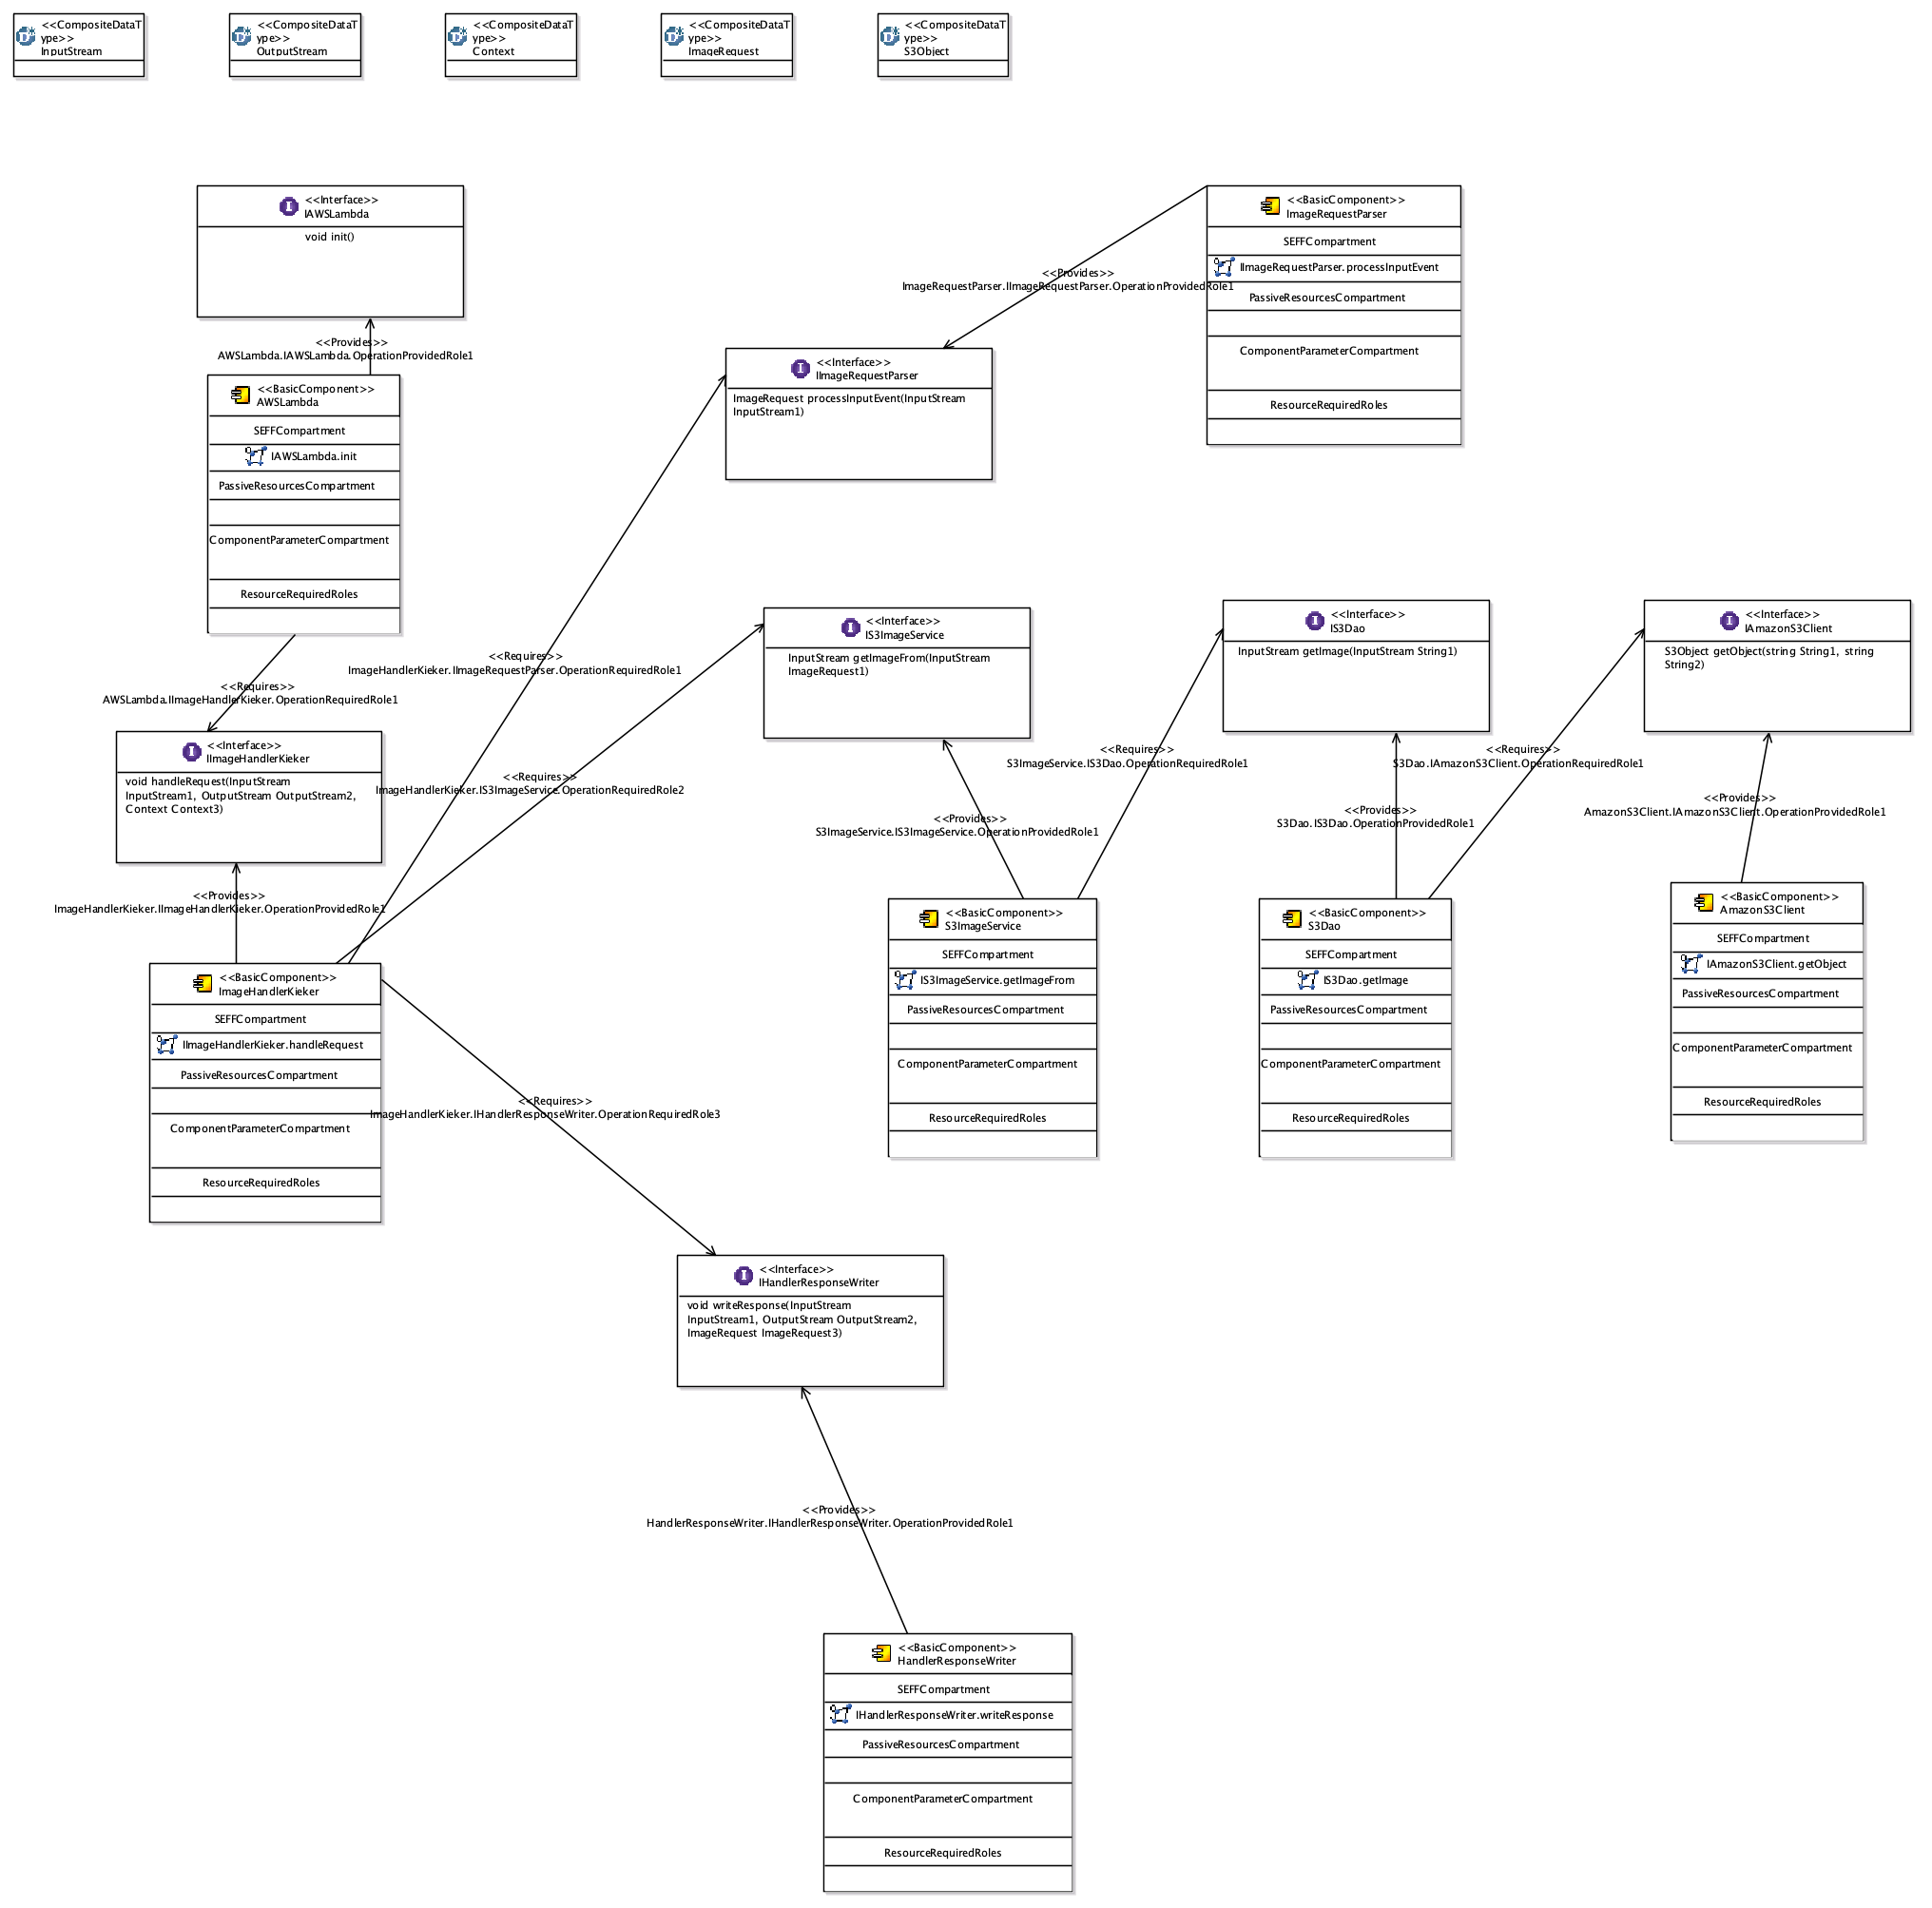
\includegraphics[width=20cm]{image-handler-extracted-repository-diagram.png}
  \caption{\emph{Image-Handler} publicando eventos de rendimiento al servicio AWS X-Ray}
  \label{fig:image-handler-pcm-model}
\end{figure}
\end{landscape}

%%%%%%%%%%%%%% Experimento 2

\subsection{Ejecución Secuencial Ininterrumpida de solicitudes de redimensionamiento}\label{sec:experimento-2}

En el experimento de la Sección \ref{sec:experimento-1} se realizaron múltiples solicitudes de redimensionamiento con el fin de extraer y crear un modelo de rendimiento, ejecutar simulaciones sobre este modelo y comparar los resultados con lo observado en una versión de \emph{Image Handler} real.

Una de las principales inquietudes durante la ejecución de funciones en la nube es  de determinar si la velocidad en la que se procesa una solicitud resulta ser baja y muestren una tendencia predecible. Los desarrolladores e implementadores necesitan evaluar esto para afinar el código fuente yla arquitectura para evitar cobros elevados por el uso de la plataforma.
De acuerdo con \cite{8360324}, una función puede pasar por dos grandes estados: uno ``fría'' y una ``caliente''. En el estado frío, la plataforma que soporta la función en la nube debe aprovisionar los recursos necesarios para ejecutar la función. Durante esta fase se pueden experimentar los tiempos de respuesta más prolongados. La fase caliente se da luego de que la plataforma que soporta la función reconoce que la función está siendo invocada constantemente y que, debido a este uso, necesita proporcionarle mayores recursos computacionales para brindar mejores tiempos de respuesta. Se espera que, en una función que se esté invocando constantemente, solamente un porcentaje muy bajo del tiempo se encuentre en estado frío y la mayor parte (mientras continúe siendo invocada) estará en estado caliente.


\subsubsection{Ejecución de solicitudes de redimensionamiento simultáneas para imágenes de tamaño menor a 500Kb}

%pic-14.jpeg (500Kb) 8:40 -> 9:05
%pic-27.jpeg (500Kb - 1Mb) 10:45 -> 1am
%pic-175.jpeg (1Mb - 2Mb) 2:16min

Para la realización de este experimento se contó con la siguiente configuración:
\begin{itemize}
    \item \emph{Sujeto de prueba:} La función Lambda IM-Simple
    \item \emph{Repositorio de imágenes:} \emph{Cluster} de 1000 imágenes de tamaño menor o igual a 500Kb alojadas en Amazon S3.
    \item \emph{Carga de trabajo:} 
    \begin{enumerate}
        \item 1000 invocaciones secuenciales de redimensionamiento de imágenes con dimensiones aleatorias a IM-Simple.
        \item 1000 invocaciones secuenciales de redimensionamient de una sola imagen a IM-Simple.
    \end{enumerate}
    \item \emph{Herramientas de medición:} Amazon Cloudwatch.
\end{itemize}

En la carga de trabajo \#1, utilizando imágenes aleatorias, la ejecución de las 1000 solicitudes de redimensionamiento fueron las mismas utilizadas para el experimento de la Sección \ref{sec:experimento-1}. 

La ejecución de las 1000 solicitudes de redimensionamiento tomó 2 horas y 36 minutos. Para la carga de trabajo \#2, utilizando una sola imagen, las 1000 solicitudes de redimensionamiento tomaron 25 minutos. Se modificó el \emph{script} en \texttt{Bash} del experimento de la Sección \ref{sec:experimento-1} para elegir aleatoriamente una imagen del \emph{cluster} de 1000 y generar 1000 solicitudes secuenciales a partir de esta con dimensiones de ancho y alto estáticas.

\begin{figure}[h]
\hspace{-1.0cm}
\begin{tikzpicture}
\begin{axis}[
    width=16cm, height=12cm,
    title={\small \textbf{1000 solicitudes de redimensionamiento en imágenes $\leq 500Kb$}},
    xlabel={\small Invocaciones a IM-Simple},
    ylabel={\small Tiempo (en $ms$)},
    xmin=-10, 
    xmax=1005,
    ymin=0, 
%    ymax=4100,
    %extra y ticks = {0.9,0.95},
    extra x tick style={tick label style={font=\footnotesize}},
    grid=major,
    grid style=dashed,
]

\addplot[mark=none,blue,smooth] table [col sep=comma] {datos/tiempos-de-respuesta-hasta-500kb-simple-2.csv};

\addplot[mark=none,red,smooth] table [col sep=comma] {datos/tiempos-de-respuesta-hasta-500kb-simple-una-imagen.csv};

\legend{\small Imágenes aleatorias, \small Imagen única} 
 
\end{axis}
\end{tikzpicture}
% Formato del caption para el índice de figuras %
\caption[hola]{1000 solicitudes de redimensionamiento en imágenes $\leq 500Kb$. La línea azul representa las solicitudes hechas utilizando imágenes aleatorias. La línea roja, las solicitudes utilizando una única imagen.}
\label{fig:1000-ejecuciones-secuenciales-500kb}
\end{figure}

En la figura \ref{fig:1000-ejecuciones-secuenciales-500kb} se muestran 1000 ejecuciones secuenciales utilizando imágenes aleatorias (línea azul) y utilizando una sola imagen (línea roja). La imagen de la línea roja es de tamaño 40Kb. Los resultados de los tiempos de respuesta muestran una tendencia marcada: la primer solicitud tomó mucho más tiempo que el resto. Una vez realizada la primer solicitud, los tiempos de respuesta de la función mejoraron considerablemente y no se observaron en las subsecuentes invocaciones tiempos de respuesta que llegaran a ser similares al primero. 


\subsubsection{Ejecución de solicitudes de redimensionamiento simultáneas para imágenes de tamaño mayor a 500Kb y menor o igual a 1Mb}

Para la realización de este experimento se contó con la siguiente configuración:
\begin{itemize}
    \item \emph{Sujeto de prueba:} La función Lambda IM-Simple
    \item \emph{Repositorio de imágenes:} \emph{Cluster} de 1000 imágenes de tamaño mayor a 500Kb y menor o igual a 1Mb alojadas en Amazon S3.
    \item \emph{Carga de trabajo:} 
    \begin{enumerate}
        \item 1000 invocaciones secuenciales de redimensionamiento de imágenes con dimensiones aleatorias a IM-Simple.
        \item 1000 invocaciones secuenciales de redimensionamient de una sola imagen a IM-Simple.
    \end{enumerate}
    \item \emph{Herramientas de medición:} Amazon Cloudwatch.
\end{itemize}

En la carga de trabajo \#1, utilizando imágenes aleatorias, la ejecución de las 1000 solicitudes de redimensionamiento fueron las mismas utilizadas para el experimento de la Sección \ref{sec:experimento-1}. 

La ejecución de las 1000 solicitudes de redimensionamiento tomó 2 horas y 36 minutos. Para la carga de trabajo \#2, utilizando una sola imagen, las 1000 solicitudes de redimensionamiento tomaron 2 horas y 30 minutos. Se modificó el \emph{script} en \texttt{Bash} del experimento de la Sección \ref{sec:experimento-1} para elegir aleatoriamente una imagen del \emph{cluster} de 1000 y generar 1000 solicitudes secuenciales a partir de esta con dimensiones de ancho y alto estáticas.

\begin{figure}[h]
\hspace{-1.5cm}
\begin{tikzpicture}
\begin{axis}[
    width=16cm, height=12cm,
    title={\small \textbf{1000 solicitudes de redimensionamiento en imágenes $500Kb \leq x \leq 1Mb$}},
    xlabel={\small Invocaciones a IM-Simple},
    ylabel={\small Tiempo (en $ms$)},
    xmin=-10, 
    xmax=1005,
    ymin=0, 
    extra x tick style={tick label style={font=\footnotesize}},
    grid=major,
    grid style=dashed,
]

\addplot[mark=none,blue,smooth] table [col sep=comma] {datos/tiempos-de-respuesta-hasta-1mb-simple-2.csv};

\addplot[mark=none,red,smooth] table [col sep=comma] {datos/tiempos-de-respuesta-hasta-1mb-simple-una-imagen.csv};
 
\legend{\small Imágenes aleatorias, \small Imagen única} 

\end{axis}
\end{tikzpicture}
\caption{1000 solicitudes de redimensionamiento en imágenes $500Kb \leq x \leq 1Mb$. La línea azul representa las solicitudes hechas utilizando imágenes aleatorias. La línea roja, las solicitudes utilizando una única imagen.}
\label{fig:1000-ejecuciones-secuenciales-1mb}
\end{figure}

En la figura \ref{fig:1000-ejecuciones-secuenciales-1mb} se muestran 1000 ejecuciones secuenciales utilizando imágenes aleatorias (línea azul) y utilizando una sola imagen (línea roja). La imagen de la línea roja es de tamaño 750Kb. Los resultados de los tiempos de respuesta muestran una tendencia marcada: la primer solicitud tomó mucho más tiempo que el resto. Una vez realizada la primer solicitud, los tiempos de respuesta de la función mejoraron considerablemente y, en el caso de las solicitudes de redimensionamiento en imágenes aleatorias, sí se logró observar un caso en el que el tiempo de respuesta fue similar al observado en la primera solicitud. En el caso de la imagen única no se observaron tiempos de respuesta que llegaran a ser similares al primero en posteriores invocaciones. 


\subsubsection{Ejecución de invocaciones de redimensionamiento simultáneas para imágenes de tamaño mayor a 1Mb y menor o igual a 2Mb}

Para la realización de este experimento se contó con la siguiente configuración:
\begin{itemize}
    \item \emph{Sujeto de prueba:} La función Lambda IM-Simple
    \item \emph{Repositorio de imágenes:} \emph{Cluster} de 1000 imágenes de tamaño mayor a 1Mb y menor o igual a 2Mb alojadas en Amazon S3.
    \item \emph{Carga de trabajo:} 
    \begin{enumerate}
        \item 1000 invocaciones secuenciales de redimensionamiento de imágenes con dimensiones aleatorias a IM-Simple.
        \item 1000 invocaciones secuenciales de redimensionamiento de una sola imagen a IM-Simple.
    \end{enumerate}
    \item \emph{Herramientas de medición:} Amazon Cloudwatch.
\end{itemize}

En la carga de trabajo \#1, utilizando imágenes aleatorias, la ejecución de las 1000 solicitudes de redimensionamiento fueron las mismas utilizadas para el experimento de la Sección \ref{sec:experimento-1}. 

La ejecución de las 1000 solicitudes de redimensionamiento tomó 2 horas y 36 minutos. Para la carga de trabajo \#2, utilizando una sola imagen, las 1000 solicitudes de redimensionamiento tomaron 2 horas y 16 minutos. Se modificó el \emph{script} en \texttt{Bash} del experimento de la Sección \ref{sec:experimento-1} para elegir aleatoriamente una imagen del \emph{cluster} de 1000 y generar 1000 solicitudes secuenciales a partir de esta con dimensiones de ancho y alto estáticas.


\begin{figure}[h]
\hspace{-1.5cm}
\begin{tikzpicture}
\begin{axis}[
    width=16cm, height=12cm,
    title={\small \textbf{1000 solicitudes de redimensionamiento en imágenes $1Mb \leq x \leq 2Mb$}},
    xlabel={\small Invocaciones a IM-Simple},
    ylabel={\small Tiempo (en $ms$)},
    xmin=-10, 
    xmax=1005,
    ymin=0, 
%    ymax=4100,
    %extra y ticks = {0.9,0.95},
    extra x tick style={tick label style={font=\footnotesize}},
    grid=major,
    grid style=dashed,
]

\addplot[mark=none,blue,smooth] table [col sep=comma] {datos/tiempos-de-respuesta-mas-de-1mb-simple-2.csv};

\addplot[mark=none,red,smooth, style={ultra thick}] table [col sep=comma] {datos/tiempos-de-respuesta-mas-de-1mb-simple-una-imagen.csv};

\legend{\small Imágenes aleatorias, \small Imagen única} 
 
\end{axis}
\end{tikzpicture}
\caption{1000 solicitudes de redimensionamiento en imágenes $1Mb \leq x \leq 2Mb$. La línea azul representa las solicitudes hechas utilizando imágenes aleatorias. La línea roja, las solicitudes utilizando una única imagen.}
\label{fig:1000-ejecuciones-secuenciales-2mb}
\end{figure}

En la figura \ref{fig:1000-ejecuciones-secuenciales-2mb} se muestran 1000 ejecuciones secuenciales utilizando imágenes aleatorias (línea azul) y utilizando una sola imagen (línea roja). La imagen de la línea roja es de tamaño 1,4Mb. Los resultados de los tiempos de respuesta muestran una tendencia similar a los casos anteriores: la primer solicitud tomó mucho más tiempo que el resto. Una vez realizada la primer solicitud, los tiempos de respuesta de la función mejoraron considerablemente y, en el caso de las solicitudes de redimensionamiento en imágenes aleatorias, sí se logró observar un caso en el que el tiempo de respuesta fue similar al observado en la primera solicitud. En el caso de la imagen única no se observaron tiempos de respuesta que llegaran a ser similares al primero en posteriores invocaciones. 

\subsubsection{Análisis de resultados}
Luego de las invocaciones de redimensionamiento tanto en imágenes aleatorias como en una sola imagen, se pudo observar que, si bien en las primeras invocaciones se experimenta mayores tiempos de respuesta, los tiempos de respuesta entregados por la función Lambda lograron bajar significativamente y en los casos de las invocaciones de redimiensionamiento en una sola imagen, estos tiempos lograron mantenerse sumamente estables.

Este comportamiento sugiere que en la invocación de una función Lambda en AWS, la plataforma subyacente primero necesita aplicar tareas de aprovisionamiento para poner a disposición la función, y, una vez que esto se realiza, la función paulatinamente pasando a un estado ``caliente'' conforme van arribando las invocaciones de redimensionamiento. Aunque la arquitectura del servicio AWS Lambda no se encuentra disponible públicamente, en árticulos en Internet y en proyectos paralelos como SAM Cli y \emph{AWS Lambda container image converter tool}\footnote{\url{https://github.com/awslabs/aws-lambda-container-image-converter}} se sugiere el uso de contenedores Docker que son provisionados con el código de la función y que se encargan de procesar las invocaciones entrantes. 

\paragraph{Relación con el modelo de rendimiento obtenido} El modelo de rendimiento obtenido y las simulaciones hechas son agnósticos a los estados ``frío'' o ``caliente'' que se muestran en las observaciones. El principal objetivo de los simuladores de PCM es el de obtener múltiples combinaciones de ejecuciones de una arquitectura de software dada, y, a menos que una comportamiento o característica de esta logre ser introducido en el modelo es que su impacto debería de verse reflejado en las simulaciones.

Si bien, en el modelo obtenido no se introdujo esto explícitamente, las mediciones muestran que los tiempos de respuesta más prolongados se corresponden con el momento en que la función estaba en estado ``frío'', por ejemplo, durantes las primeras invocaciones. Si se toma como referencia el primer experimento ejecutado en la Sección \ref{sec:experimento-1}, invocaciones de redimensionamiento en imágenes menores o iguales a 500Kb, en la figura \ref{fig:comparacion-imsimple-palladio-500kb}, la primera medición a IM-Simple dió como resultado 4.1s y las subsecuentes 999 invocaciones bajaron a 1,6 segundos o menos; muchas de ellas incluso fueron menores a medio segundo. En los resultados de este experimento, existe un 95\% de probablidades que los tiempos de respuesta de las invocaciones sean de 1,6 segundos o menos, lo que, visto desde otro ángulo, quiere decir que existe un 5\% de probabilidad que los tiempos de respuesta de las  invocaciones tomen entre 1,6 y 4 segundos en ser procesadas. Ahora bien, aunque 5\% parece ser una probabilidad muy alta y que no refleja lo visto en las mediciones, cuando se vuelve a los resultados de las simulaciones se observa que hay probabilidad mayor al 99\% de que una invocación de redimensionamiento tenga un tiempo de respuesta igual o menor a 2 segundos. Esto quiere decir que hay una probabilidad de menos del 1\% de que una invocación a la función Lambda tome entre 2 y 4 segundos en ser procesada. En el caso de las simulaciones de la Figura \ref{fig:comparacion-imsimple-palladio-500kb} solamente 6 casos muestran tiempos de respuesta de entre 2 y 4 segundos lo que representa un 0.006\% del total de las simulaciones realizadas.

Lo anterior señala que, para el caso de \emph{Image Handler}, las simulaciones con los tiempos de respuesta más prolongados representan una cantidad muy pequeña de la totalidad de los casos y que, estos casos se pueden convertir en potenciales escenarios de la función Lambda en estado frío. Las simulaciones muestran que a pesar del impacto que tienen estos escenarios en las invocaciones, estos realmente no llegan afectar el comportamiento general de la función Lambda. 

Con respecto a los resultados de este experimento y su relación con los escenarios de invocaciones de redimiensionamiento en imágenes de tamaño de 500Kb y menor o igual a 1Mb, e imágenes de tamaño de 1Mb y menor a 2Mb, expuestas en la Sección \ref{sec:experimento-1}, se puede emplear un análisis similar: las simulaciones que reportan los tiempos de respuesta más prolongados tienen el potencial de caracterizar las ejecuciones de la función en estado ``frío''.

%%%%%%%%%%%%%% Experimento 2
\subsection{Variación del intervalo de las invocaciones de redimensionamiento}

Este experimento se plantea como una variación del expuesto en la Sección \ref{sec:experimento-2}, donde se evaluaba el efecto de las invocaciones simultáneas a la función Lambda. Acá se plantea variar el intervalo entre invocaciones a la función Lambda con el fin de valorar los efectos en el comportamiento de la función y si el modelo obtenido en la Sección \ref{sec:experimento-1} contribuye a explicar algo de lo observado; en particular si los intervalos entre las invocaciones hacen que el rendimiento de la función se considere ``fría'' o ``caliente'' en algún punto.

\subsubsection{Estrategia de intervalo de invocaciones a \emph{Image Handler}}
Para evaluar los efectos de los intervalos de lanzamiento en las invocaciones a \emph{Image Handler}, se propone la ejecución de un número de invocaciones simultáneas (una ráfaga), luego entrar en un tiempo de espera y luego, aplicar otra ráfaga de invocaciones. 

El tiempo de espera entre ráfagas se irá incrementando al doble del tiempo de espera anterior. Por ejemplo, si el primer tiempo de espera es de 2 minutos, el siguiente será de 4 minutos, luego 8, 16, 32 minutos y así sucesivamente. Para este experimento se propone utilizar tiempos de espera inicial de 10 minutos para luego aumentarlo en subsecuentes ráfagas de invocaciones.

\subsubsection{Ejecución de ráfagas de invocaciones de redimensionamiento para imágenes de tamaño menor a 500Kb}

Para la realización de este experimento se utilizó la siguiente configuración base:
\begin{itemize}
    \item \emph{Sujeto de prueba:} La función Lambda IM-XRay.
    \item \emph{Repositorio de imágenes:} \emph{Cluster} de 1000 imágenes de tamaño menor o a 500Kb alojadas en Amazon S3.
    \item \emph{Carga de trabajo:} 100 invocaciones secuenciales de redimensionamiento de imágenes con dimensiones aleatorias a IM-XRay seguido de un tiempo de espera de 10, 20 y 40 minutos.      
    \item \emph{Herramientas de medición:} Amazon Cloudwatch y Amazon X-Ray.
\end{itemize}
 
De acuerdo con lo observado en los experimentos anteriores, luego de la primera invocación, las subsiguientes hacen que la función entre en un estado ``caliente''. Por esta razón, ejercitar la función con una ráfaga de 100 invocaciones haría que se logre llegar a este estado fácilmente.

A diferencia de los experimentos anteriores, se utiliza la versión de IM-XRay en lugar de IM-Simple. La razón es que se quiere sacar provecho a las herramientas de monitoreo de AWS X-Ray para determinar si la función pasa de un estado \emph{frío $\rightarrow$ caliente $\rightarrow$ frío} y determinar el impacto de este cambio en el tiempo de respuesta.

\subsubsection{Variando el intervalo de las invocaciones de redimensionamiento en imágenes $\leq 500Kb$}\label{sec:rafagas-hasta-500kb}

La Figura \ref{fig:rafagas-hasta-500kb} muestra 400 invocaciones de redimensionamiento en imágenes menores a 500Kb divididas en 100 ráfagas cada una. En la primer ráfaga la función se encuentra en estado ``frío'', sucede el aprovisionamiento inicial. Luego de esta primer invocación la función va entrando paulatinamente en estado ``caliente'' y se logra observar que para la mayoría de los casos las invocaciones de redimensionamiento no llegan a tomar más de 1,5 segundos. El tiempo promedio de ejecución de una ráfaga fue de 2 minutos y 45 segundos.

\begin{figure}
\hspace{-1.0cm}
\begin{tikzpicture}
\begin{axis}[
    width=16cm, height=12cm,
    title={\small \textbf{4 ráfagas de 100 invocaciones de redimensionamiento en imágenes $\leq 500Kb$}},
    xlabel={\small Invocaciones a IM-XRay},
    ylabel={\small Tiempo (en $ms$)},
    xmin=-10, 
    xmax=535,
    ymin=0, 
%    ymax=6000,
%    extra x ticks = {90,165},
    extra x tick style={tick label style={font=\footnotesize}},
    grid=major,
    grid style=dashed,
]

\addplot[mark=none,blue,smooth] table [col sep=comma] {datos/hasta-500kb-rafagas-bck-1.csv};
\addplot[color=red, mark=none, dashed, opacity=0.5] coordinates {(103,0)(103,10000)(117,10000)(117,0)};
\addplot[mark=none,blue,smooth] table [col sep=comma] {datos/hasta-500kb-rafagas-bck-2.csv};
\addplot[color=red, mark=none, dashed, opacity=0.5] coordinates {(223,0)(223,10000)(257,10000)(257,0)};
\addplot[mark=none,blue,smooth] table [col sep=comma] {datos/hasta-500kb-rafagas-bck-3.csv};
\addplot[color=red, mark=none, dashed, opacity=0.5] coordinates {(362,0)(363,10000)(429,10000)(429,0)};
\addplot[mark=none,blue,smooth] table [col sep=comma] {datos/hasta-500kb-rafagas-bck-4.csv};

%\legend{\small Imágenes aleatorias, \small Imagen única} 
 
\end{axis}
\end{tikzpicture}
\caption{El espacio delimitado por la línea punteada roja representa 10 minutos de inactividad entre la primer ráfaga y la segunda. El segundo espacio delimitado por la línea punteada roja representa 20 minutos de inactividad entre la segunda y la tercera ráfaga.}
\label{fig:rafagas-hasta-500kb}
\end{figure}

En la segunda ráfaga, luego de 10 minutos, la función no experimenta un tiempo de respuesta inicial similar al de la primer ráfaga. Esto quiere decir que pasados 10 minutos de inactividad entre la primer y segunda ráfaga, la función continua en estado caliente.

En la tercer ráfaga, luego de 20 minutos de haberse ejecutado la última invocación de redimensionamiento de la ráfaga anterior, sí se llega observar un tiempo de respuesta inicial alto. AWS X-Ray reporta que en esta invocación inicial se tuvo que re-aprovisionar la función, lo que sugiere que, durante los 20 minutos de inactividad entre una ráfaga y otra, la función fue pasando progresivamente a un estado ``frío'' debido a que la plataforma pudo determinar que el nivel de actividad de la función (cantidad de invocaciones) fue decreciendo hasta un punto en donde no detectó actividad alguna.

La última ráfaga también experimentó un tiempo de respuesta inicial alto. Esta vez un poco mayor al de la ráfaga anterior pero menor a la de la primer ráfaga. Hubo 40 minutos de inactividad entre la tercera ráfaga y la cuarta. 

\subsubsection{Variando el intervalo de las invocaciones de redimensionamiento en imágenes $500Kb \leq x \leq 1Mb$}

Se hizo el mismo ejercicio que en la Sección \ref{sec:rafagas-hasta-500kb}. La Figura \ref{fig:rafagas-hasta-1mb} muestra los resultados de la ejecución de 5 ráfagas de 100 invocaciones cada una. El tiempo promedio de ejecución de una ráfaga fue de 9 minutos y 15 segundos. En la primera invocación de la primer ráfaga se obtuvo un tiempo de respuesta alto (función en estado frío). En la segunda ráfaga no se observó tiempos de respuesta elevados debido a que la función se encontraba en estado ``caliente''. 

\begin{figure}
\hspace{-1cm}
\begin{tikzpicture}
\begin{axis}[
    width=16cm, height=12cm,
    title={\small \textbf{5 ráfagas de 100 invocaciones de redimensionamiento en imágenes $500Kb \leq x \leq 1Mb$}},
    xlabel={\small Invocaciones a IM-XRay},
    ylabel={\small Tiempo (en $ms$)},
    xmin=-10, 
    xmax=775,
    ymin=0, 
    ymax=14000,
%    extra x ticks = {90,165},
    extra x tick style={tick label style={font=\footnotesize}},
    grid=major,
    grid style=dashed,
]

\addplot[mark=none,blue,smooth] table [col sep=comma] {datos/hasta-1mb-rafagas-1.csv};
\addplot[color=red, mark=none, dashed, opacity=0.5] coordinates {(103,0)(103,10000)(117,10000)(117,0)};
\addplot[mark=none,blue,smooth] table [col sep=comma] {datos/hasta-1mb-rafagas-2.csv};
\addplot[color=red, mark=none, dashed, opacity=0.5] coordinates {(223,0)(223,10000)(257,10000)(257,0)};
\addplot[mark=none,blue,smooth] table [col sep=comma] {datos/hasta-1mb-rafagas-3.csv};
\addplot[color=black, mark=none, dashed, style={ultra thick}] coordinates {(260,8082)(260,14000)};
\addplot[color=red, mark=none, dashed, opacity=0.5] coordinates {(362,0)(363,10000)(429,10000)(429,0)};
\addplot[mark=none,blue,smooth] table [col sep=comma] {datos/hasta-1mb-rafagas-4.csv};
\addplot[color=black, mark=none, dashed, style={ultra thick}] coordinates {(434,9356)(434,14000)};
\addplot[color=red, mark=none, dashed, opacity=0.5] coordinates {(535,0)(535,10000)(671,10000)(671,0)};
\addplot[mark=none,blue,smooth] table [col sep=comma] {datos/hasta-1mb-rafagas-5.csv};
 
\end{axis}
\end{tikzpicture}
\caption{El espacio delimitado por la línea punteada roja representa 10 minutos de inactividad entre la primer ráfaga y la segunda. El espacio delimitado por la línea punteada verde representa 20 minutos de inactividad entre la segunda y la tercera ráfaga.}
\label{fig:rafagas-hasta-1mb}
\end{figure}

En la primera invocación de la tercera y cuarta ráfaga, AWS X-Ray reportó que en ambas hubo que re-aprovisionar la función. Es decir, el tiempo de inactividad entre la segunda ráfaga (20 minutos) y entre la tercera y la cuarta (40 minutos) fue suficiente para que la plataforma volviera a marcar la función como fría de nuevo. Lo interesante de estas dos primeras invocaciones, es que, a pesar que la plataforma tuvo que volver a re-aprovisionar la función, los tiempos de respuesta reportados fueron mucho más bajos que el de la invocación inicial de la primer ráfaga. En la Tabla \ref{table:rafagas-hasta-1mb-tiempos-primera-invocacion} se pueden ver los tiempos de respuesta de las primeras invocaciones de cada ráfaga.

\begin{table}
    \centering
    \begin{tabular}{l|r}
        \toprule[1.5pt]
        \multicolumn{2}{c}{\textbf{Entre 500Kb a 1Mb}} \\
        \midrule
        Ráfaga  & Tiempo de 1º invocación \\
        \midrule
        \#1  & 13s \\
        \#2  & N.A. \\        
        \#3  & 8s \\        
        \#4  & 9s \\        
        \#5  & 11s \\                                
        \bottomrule[1.5pt]
    \end{tabular}
    \caption{Tiempo de respuesta de la primer invocación de redimensionamiento en cada ráfaga.}
    \label{table:rafagas-hasta-1mb-tiempos-primera-invocacion}
\end{table}

En la quinta ráfaga, el tiempo de respuesta de la primera invocación se elevó de nuevo. El tiempo de inactividad entre la cuarta ráfaga y la quinta fue de 80 minutos. 

Debido a que los tiempos iniciales de la tercera y cuarta ráfaga fueron bajos (aunque AWS X-Ray reporta que para cada uno de ellos fue necesaria re-aprovisionar la función), fue que se la ejecución de una quita ráfaga se hizo necesaria con el fin de validar que, conforme los tiempos de inactividad entre ráfagas aumenta, el tiempo de respuesta de la primera invocación también aumenta. 

\subsubsection{Variando el intervalo de las invocaciones de redimensionamiento en imágenes $1Mb \leq x \leq 2Mb$}

Para este caso, el tiempo promedio de ejecución de una ráfaga fue de 13 minutos y 15 segundos. En la ejecución de cada ráfaga, AWS X-Ray reportó que fue necesario re-aprovisionar la función cuando se ejecutó la primera invocación de cada ráfaga. En la Figura \ref{fig:rafagas-hasta-2mb} se muestran los resultados de la ejecución de las cuatro ráfagas.

\begin{figure}
\hspace{-1.5cm}
\begin{tikzpicture}
\begin{axis}[
    width=16cm, height=12cm,
    title={\small \textbf{4 ráfagas de 100 invocaciones de redimensionamiento en imágenes $1Mb \leq x \leq 2Mb$}},
    xlabel={\small Invocaciones a IM-XRay},
    ylabel={\small Tiempo (en $ms$)},
    xmin=-10, 
    xmax=535,
    ymin=0, 
    ymax=16000,
%    extra x ticks = {90,165},
    extra x tick style={tick label style={font=\footnotesize}},
    grid=major,
    grid style=dashed,
]

\addplot[mark=none,blue,smooth] table [col sep=comma] {datos/hasta-2mb-rafagas-1.csv};
\addplot[color=red, mark=none, dashed, opacity=0.5] coordinates {(103,0)(103,10000)(117,10000)(117,0)};
\addplot[mark=none,blue,smooth] table [col sep=comma] {datos/hasta-2mb-rafagas-2.csv};
\addplot[color=red, mark=none, dashed, opacity=0.5] coordinates {(223,0)(223,10000)(257,10000)(257,0)};
\addplot[mark=none,blue,smooth] table [col sep=comma] {datos/hasta-2mb-rafagas-3.csv};
\addplot[color=red, mark=none, dashed, opacity=0.5] coordinates {(362,0)(363,10000)(429,10000)(429,0)};
\addplot[mark=none,blue,smooth] table [col sep=comma] {datos/hasta-2mb-rafagas-4.csv};
 
\end{axis}
\end{tikzpicture}
\caption{El espacio delimitado por la línea punteada roja representa 10 minutos de inactividad entre la primer ráfaga y la segunda. El espacio delimitado por la línea punteada verde representa 20 minutos de inactividad entre la segunda y la tercera ráfaga.}
\label{fig:rafagas-hasta-2mb}
\end{figure}

Los tiempos de respuesta de las primeras invocaciones de cada ráfaga resultaron ser más similares entre sí y, también se pudo observar que cuando existen tiempos de inactivad más prolongados, como el que entre la ráfaga tres y la cuando que es de 40 minutos, a la siguiente invocación le toma un mayor tiempo de respuesta que la primer invocación de la ráfaga anterior.

\subsubsection{Análisis de resultados}
La principal observación que arrojó este experimento es que conforme van aumentando los tiempos de inactividad en la función Lambda, también van aumentando los tiempos de respuesta entregados por la primera invocación luego de este tiempo de inactividad. 

De acuerdo con \cite{cold-starts-aws-lambda-1}, una vez que una función ha sido instalada en la plataforma, la primer invocación debe de pasar por el proceso de aprovisionamiento. Luego de que esta primer invocación es procesada, la función pasa a un estado activo o ``caliente'' y el contenedor que la soporta se puede reutilizar para subsecuentes invocaciones. Cuando se detecta que la función se vuelve inactiva o ``fría'', el contenedor que la soporta se vuelve candidato a ser ``reciclado'' para ser utilizado por otra función que lo necesite.

Si bien no hay un tiempo límite definido para decidir cuándo el contenedor va a ser reciclado o no, los resultados de este experimento y los expuestos en \cite{cold-starts-aws-lambda-1} y \cite{cold-starts-aws-lambda-2} demuestran que entre mayor sean los tiempos de inactividad de una función, mayor será la probabilidad de que el contenedor que la soporta sea reciclado y que, cuando se vuelva a invocar a la función, se experimente un tiempo de respuesta mayor al promedio debido al proceso de aprovisionamiento. 

Según las mediciones en \cite{cold-starts-aws-lambda-1}, el tiempo de vida de un contenedor no parece darse en forma determinística pero se estima que está entre los 25 a 65 minutos. Una contenedor inactivo casi siempre se mantiene vivo por 25 minutos, luego de eso la probabilidad de que sea desechado crece lentamente y llega a alcanzar el 100\% luego de alrededor de 1 hora luego de la última invocación.

\paragraph{Relación con el modelo de rendimiento obtenido} En el experimento de la Sección \ref{sec:experimento-1} se obtuvo un modelo de rendimiento a partir una sola ráfaga invocaciones secuenciales de redimensionamiento. No se introdujo tiempos de inactividad. 

Aquí, aunque se introducen tiempos de inactividad entre ráfagas, se presenta una tendencia que se ha repetido a lo largo de los tres experimentos ejecutados hasta este momento: las primeras invocaciones reportan mayores tiempos de respuesta, especialmente la primera invocación, y conforme la función va recibiendo más y más invocaciones, su tiempo de respuesta tiende a bajar considerablemente. Esta es una característica que el modelo obtenido logró reconocer y, de igual manera como en los experimentos anteriores, las invocaciones en donde los tiempos de respuesta fueron mayores representan un porcentaje muy bajo ($\approx$ 1\%) del total de invocaciones en una ráfaga, por lo que cuando el modelo reporte invocaciones con tiempos de respuesta alto se puede afirmar para el caso de \emph{Image Handler} que estas invocaciones serán muy pocas y que probablemente representen momentos en donde la función tuvo que pasar forzozamente de un estado ``frío'' a uno ``caliente''.


En PCM, el comportamiento asociado a las invocaciones basadas en ráfagas y tiempos de inactividad podría llegar a ser introducido con un modelo de uso personalizado el cual pueda tomar en cuenta las particularidades del cómo es que una arquitectura de software puede ser potencialmente utilizada pero, la forma en la que PCM reporta los resultados de las simulaciones es la misma independientemente del modelo de uso (o de cualquier otro modelo) utilizado. Es por esto que, en términos de resultados, PCM siempre va a entregar resultados basados en la probabilidad de que una determinada simulación se ejecute en una arquitectura dada. Lo anterior se usa para aclarar que mientras se utilice PCM para ejecutar simulaciones utilizando el esquema de ráfaga/tiempo de espera, los resultados obtenidos no vendrán dados de forma específica para cada ráfaga ejecutada, sino más bien serán presentados de forma general.

\subsection{Comparación de \texttt{SAM CLI} con observaciones reales}

\begin{figure}
\hspace{-1cm}
\begin{tikzpicture}
	\begin{axis}[
	width=16cm, height=12cm, xmin=0, ymin=0,
	xmax=1010, 
%	ymax=14500,
	title={\textbf{\emph{Image Handler vs} \texttt{SAM CLI}: redimensionamiento en imágenes de tamaño $\leq 500Kb$}},
	xlabel={\small Número de ejecución de solicitud de redimensionamiento},
	ylabel={\small Milisegundos},
	grid=major, grid style=dashed, label style={font=\small},
	tick label style={font=\footnotesize},
	scatter/classes={%
		a={mark=square*,blue},%
		b={mark=square*,red},%
		c={mark=o,draw=black}}]			
	\addplot[scatter,only marks,%
		scatter src=explicit symbolic]%
	table[meta=label, col sep=comma] {datos/xy-sam-data-500kb.csv};
	\legend{Solicitudes a \emph{Image Handler}, Solicitudes en \texttt{SAM CLI}}
	\end{axis}
\end{tikzpicture}
\caption{Solicitudes de redimensionamiento de imágenes de tamaño $1Mb \leq x \leq 2Mb$}
\label{fig:comparacion-sam-500kb}
\end{figure}


\begin{figure}
\hspace{-1cm}
\begin{tikzpicture}
	\begin{axis}[
	width=16cm, height=12cm, xmin=0, ymin=0,
	xmax=1010, 
%	ymax=14500,
	title={\textbf{\emph{Image Handler vs} \texttt{SAM CLI}: redimensionamiento en imágenes de tamaño $500Kb \leq x \leq 1Mb$}},
	xlabel={\small Número de ejecución de solicitud de redimensionamiento},
	ylabel={\small Milisegundos},
	grid=major, grid style=dashed, label style={font=\small},
	tick label style={font=\footnotesize},
	scatter/classes={%
		a={mark=square*,blue},%
		b={mark=square*,red},%
		c={mark=o,draw=black}}]			
	\addplot[scatter,only marks,%
		scatter src=explicit symbolic]%
	table[meta=label, col sep=comma] {datos/xy-sam-data-1mb.csv};
	\legend{Solicitudes a \emph{Image Handler}, Solicitudes en \texttt{SAM CLI}}
	\end{axis}
\end{tikzpicture}
\caption{Solicitudes de redimensionamiento de imágenes de tamaño $500kb \leq x \leq 1Mb$}
\label{fig:comparacion-sam-1mb}
\end{figure}


\begin{figure}
\hspace{-1cm}
\begin{tikzpicture}
	\begin{axis}[
	width=16cm, height=12cm, xmin=0, ymin=0,
	xmax=1010, 
%	ymax=14500,
	title={\textbf{\emph{Image Handler vs} \texttt{SAM CLI}: redimensionamiento en imágenes de tamaño $500Kb \leq x \leq 1Mb$}},
	xlabel={\small Número de ejecución de solicitud de redimensionamiento},
	ylabel={\small Milisegundos},
	grid=major, grid style=dashed, label style={font=\small},
	tick label style={font=\footnotesize},
	scatter/classes={%
		a={mark=square*,blue},%
		b={mark=square*,red},%
		c={mark=o,draw=black}}]			
	\addplot[scatter,only marks,%
		scatter src=explicit symbolic]%
	table[meta=label, col sep=comma] {datos/xy-sam-data-2mb.csv};
	\legend{Solicitudes a \emph{Image Handler}, Solicitudes en \texttt{SAM CLI}}
	\end{axis}
\end{tikzpicture}
\caption{Solicitudes de redimensionamiento de imágenes de tamaño $1Mb \leq x \leq 2Mb$}
\label{fig:comparacion-sam-2mb}
\end{figure}





% Rafaga 500Kb en promedio 2min, 45seg
% Rafaga 1Mb en promedio 9 min, 15 seg
% Rafaga 2Mb en promedio 13 min, 15 seg



%\hspace{-3cm}
%\begin{tikzpicture}
%\begin{axis}[
%    width=18cm, height=15cm,
%    title={\textbf{1000 Simulaciones: Función de probabilidad acumulada para los tres escenarios de pruebas }},
%    xlabel={Segundos},
%    ylabel={Probabilidad acumulada},
%    xmin=0, xmax=12,
%    ymin=0, ymax=1.05,
%    extra y ticks = {0.9,0.95},
%    extra x ticks = {1.6, 10.135},
%    extra x tick style={tick label style={font=\footnotesize}},    
%%    legend pos=north east,
%	legend style={at={(0.5,-0.15)},
%		anchor=north,legend columns=-1},
%    grid=major,
%    grid style=dashed,
%]
%
%\addplot[mark=none,blue,smooth] table [col sep=comma] {datos/hasta-500kb-cdf.csv};
%\addplot[mark=none,green,smooth] table [col sep=comma] {datos/hasta-1mb-cdf.csv};
%\addplot[mark=none,orange,smooth] table [col sep=comma] {datos/mas-1mb-cdf.csv};
%
%\coordinate (a) at (axis cs:1.6, 0.95);
%%\draw[blue, dashed, thick](a -| current plot begin) -- (a);
%\draw[blue, dashed, thick](a |- current plot begin) -- (a);
%
%\coordinate (b) at (axis cs:8.0, 0.95);
%%\draw[red, dashed, thick](b -| current plot begin) -- (b);
%\draw[green, dashed, thick](b |- current plot begin) -- (b);
%
%\coordinate (b) at (axis cs:10.135, 0.95);
%%\draw[red, dashed, thick](b -| current plot begin) -- (b);
%\draw[orange, dashed, thick](b |- current plot begin) -- (b);
% 
%\legend{Hasta 500Kb, De 500Kb a 1Mb, Mayor a 1Mb} 
% 
%\end{axis}
%\end{tikzpicture}
%
%
%\hspace{-3.0cm}
%\begin{tikzpicture}
%\begin{axis}[
%  width=19cm, height=8.3cm,
%  title style={align=center},
%  title={Distribución de los tiempos de respuesta en solicitudes de redimensionamiento\\de imágenes de tamaño $\leq 500Kb$ en las simulaciones de Palladio},
%  ylabel={Solicitudes de redimensionamiento},
%  xmin=0, ymin=0, xmax=4000,
%  ybar interval,
%  xtick=data,
%  xticklabel interval boundaries,
%  x tick label style={rotate=45,anchor=east}
%  ],
%	\addplot+[hist={bins=10}]
%		table[col sep=comma, y index=0] {datos/tiempos-de-respuesta-hasta-500kb-palladio.csv};
%\legend{Tiempos de respuesta (En $ms$)}
%\end{axis}
%\end{tikzpicture}
%
%\hspace{-3.0cm}
%\begin{tikzpicture}
%\begin{axis}[
%  width=19cm, height=8.3cm,
%  title style={align=center},
%  title={Distribución de los tiempos de respuesta en solicitudes de redimensionamiento\\de imágenes de tamaño $\leq 500Kb$ en \emph{Image Handler}},
%  ylabel={Solicitudes de redimensionamiento},
%  xmin=0, ymin=0, xmax=4020,
%  ybar interval,
%  xtick=data,
%  xticklabel interval boundaries,
%  x tick label style={rotate=45,anchor=east}
%  ],
%	\addplot+[fill=red!70!white,hist={bins=10}]
%		table[col sep=comma, y index=0] {datos/tiempos-de-respuesta-hasta-500kb-simple.csv};
%\legend{Tiempos de respuesta (En $ms$)}
%\end{axis}
%\end{tikzpicture}
%
%
%% XY PLOT 1
%\hspace{-3cm}
%\begin{tikzpicture}
%	\begin{axis}[
%	width=19cm, height=15cm, xmin=0, ymin=0,
%	xmax=1010, ymax=4500,
%	title={\textbf{1000 Solicitudes de redimensionamiento de imágenes de tamaño $\leq 500Kb$}},
%	xlabel={Número de ejecución de solicitud de redimensionamiento},
%	ylabel={Milisegundos},
%	grid=major, grid style=dashed, label style={font=\small},
%%	extra y ticks={400,600},
%%	extra y tick labels={PP, PIM},
%   extra y tick style={%
%     color=green,
%    },	
%	tick label style={font=\footnotesize},
%	scatter/classes={%
%		a={mark=square*,blue},%
%		b={mark=square*,red},%
%		c={mark=o,draw=black}}]			
%		
%%  \addplot[green,sharp plot,update limits=false] 
%%	coordinates {(0,500) (500,500) (1000,500)} 
%%	node[above] at (axis cs:400,500) {Houses};		
%		
%	\addplot[scatter,only marks,%
%		scatter src=explicit symbolic]%
%	table[meta=label, col sep=comma] {datos/xy-data-hasta-500kb.csv};
%	
%	
%	\legend{Simulaciones de Palladio, Solicitudes a \emph{Image Handler}}
%	\end{axis}
%\end{tikzpicture}

%% --------------------------------------------------

%\hspace{-3.0cm}
%\begin{tikzpicture}
%\begin{axis}[
%  width=19cm, height=8.3cm,
%  title style={align=center},
%  title={Distribución de los tiempos de respuesta en solicitudes de redimensionamiento\\de imágenes de tamaño $500Kb \leq x \leq 1Mb$ en las simulaciones de Palladio},
%  ylabel={Solicitudes de redimensionamiento},
%  xmin=0, ymin=0, xmax=9300,
%  ybar interval,
%  xtick=data,
%  xticklabel interval boundaries,
%  x tick label style={rotate=45,anchor=east}
%  ],
%	\addplot+[hist={bins=10}]
%		table[col sep=comma, y index=0] {datos/tiempos-de-respuesta-hasta-1mb-palladio.csv};
%\legend{Tiempos de respuesta (En $ms$)}
%\end{axis}
%\end{tikzpicture}
%
%\hspace{-3.0cm}
%\begin{tikzpicture}
%\begin{axis}[
%  width=19cm, height=8.3cm,
%  title style={align=center},
%  title={Distribución de los tiempos de respuesta en solicitudes de redimensionamiento\\de imágenes de tamaño $500Kb \leq x \leq 1Mb$ en \emph{Image Handler}},
%  ylabel={Solicitudes de redimensionamiento},
%  xmin=0, ymin=0, xmax=8500,
%  ybar interval,
%  xtick=data,
%  xticklabel interval boundaries,
%  x tick label style={rotate=45,anchor=east}
%  ],
%	\addplot+[fill=red!70!white,hist={bins=10}]
%		table[col sep=comma, y index=0] {datos/tiempos-de-respuesta-hasta-1mb-simple.csv};
%\legend{Tiempos de respuesta (En $ms$)}
%\end{axis}
%\end{tikzpicture}
%
%\hspace{-2cm}
%\begin{tikzpicture}
%	\begin{axis}[
%	width=18cm, height=15cm, xmin=0, ymin=0,
%	xmax=1010, 
%	ymax=9500,
%	title={\textbf{Solicitudes de redimensionamiento de imágenes de tamaño $500Kb \leq x \leq 1Mb$}},
%	xlabel={Número de ejecución de solicitud de redimensionamiento},
%	ylabel={Milisegundos},
%	grid=major, grid style=dashed, label style={font=\small},
%%	extra y ticks={400,600},
%%	extra y tick labels={PP, PIM},
%%   extra y tick style={%
%%     color=green,
%%    },	
%	tick label style={font=\footnotesize},
%	scatter/classes={%
%		a={mark=square*,blue},%
%		b={mark=square*,red},%
%		c={mark=o,draw=black}}]			
%	\addplot[scatter,only marks,%
%		scatter src=explicit symbolic]%
%	table[meta=label, col sep=comma] {datos/xy-data-hasta-1mb.csv};
%	\legend{Simulaciones de Palladio, Solicitudes a \emph{Image Handler}}
%	\end{axis}
%\end{tikzpicture}
%
%\hspace{-3.0cm}
%\begin{tikzpicture}
%\begin{axis}[
%  width=19cm, height=15cm,
%  title={\textbf{Distribución del tamaño de imágenes de tamaño $500Kb \leq x \leq 1Mb$}},
%  ylabel={Cantidad de imágenes},
%  xmin=0, ymin=0, xmin=500, xmax=1024,
%  ybar interval,
%  xtick=data,
%  xticklabel interval boundaries,
%  x tick label style={rotate=45,anchor=east}  
%  ],
%	\addplot+[hist={bins=10}]
%		table[col sep=comma, y index=0] {datos/tamannos-cluster-b.csv};
%\legend{Tamaño de imágenes}
%\end{axis}
%\end{tikzpicture}
%
%%% --------------------------------------------------
%
%\hspace{-3.0cm}
%\begin{tikzpicture}
%\begin{axis}[
%  width=19cm, height=8.3cm,
%  title style={align=center},
%  title={Distribución de los tiempos de respuesta en solicitudes de redimensionamiento\\de imágenes de tamaño $1Mb \leq x \leq 2Mb$ en las simulaciones de Palladio},
%  ylabel={Solicitudes de redimensionamiento},
%  xmin=3700, ymin=0, xmax=14000,
%  ybar interval,
%  xtick=data,
%  xticklabel interval boundaries,
%  x tick label style={rotate=45,anchor=east}
%  ],
%	\addplot+[hist={bins=10}]
%		table[col sep=comma, y index=0] {datos/tiempos-de-respuesta-mas-de-1mb-palladio.csv};
%\legend{Tiempos de respuesta (En $ms$)}
%\end{axis}
%\end{tikzpicture}
%
%\hspace{-2.5cm}
%\begin{tikzpicture}
%\begin{axis}[
%  width=19cm, height=8.3cm,
%  title style={align=center},
%  title={Distribución de los tiempos de respuesta en solicitudes de redimensionamiento\\de imágenes de tamaño $1Mb \leq x \leq 2Mb$ en \emph{Image Handler}},
%  ylabel={Solicitudes de redimensionamiento},
%  xmin=3900, ymin=0, xmax=10000,
%  ybar interval,
%  xtick=data,
%  xticklabel interval boundaries,
%  x tick label style={rotate=45,anchor=east}
%  ],
%	\addplot+[fill=red!70!white,hist={bins=10}]
%		table[col sep=comma, y index=0] {datos/tiempos-de-respuesta-mas-de-1mb-simple.csv};
%\legend{Tiempos de respuesta (En $ms$)}
%\end{axis}
%\end{tikzpicture}
%
%
%% XY Plot 3
%\hspace{-3cm}
%\begin{tikzpicture}
%	\begin{axis}[
%	width=19cm, height=15cm, xmin=0, ymin=0,
%	xmax=1010, 
%	ymax=14500,
%	title={\textbf{Solicitudes de redimensionamiento de imágenes de tamaño $1Mb \leq x \leq 2Mb$}},
%	xlabel={Número de ejecución de solicitud de redimensionamiento},
%	ylabel={Milisegundos},
%	grid=major, grid style=dashed, label style={font=\small},
%	tick label style={font=\footnotesize},
%	scatter/classes={%
%		a={mark=square*,blue},%
%		b={mark=square*,red},%
%		c={mark=o,draw=black}}]			
%	\addplot[scatter,only marks,%
%		scatter src=explicit symbolic]%
%	table[meta=label, col sep=comma] {datos/xy-data-mas-de-1mb.csv};
%	\legend{Simulaciones de Palladio, Solicitudes a \emph{Image Handler}}
%	\end{axis}
%\end{tikzpicture}
%
%\hspace{-3.0cm}
%\begin{tikzpicture}
%\begin{axis}[
%  width=19cm, height=15cm,
%  title={\textbf{Distribución del tamaño de imágenes de tamaño $1Mb \leq x \leq 2Mb$}},
%  ylabel={Cantidad de imágenes},
%  xmin=0, ymin=0, xmin=1000, xmax=2048,
%  ybar interval,
%  xtick=data,
%  xticklabel interval boundaries,
%  x tick label style={rotate=45,anchor=east}  
%  ],
%	\addplot+[hist={bins=10}]
%		table[col sep=comma, y index=0] {datos/tamannos-cluster-c.csv};
%\legend{Tamaño de imágenes}
%\end{axis}
%\end{tikzpicture}
%
%%% --------------------------------------------------
%
%\hspace{-4cm}
%\begin{table}
%    \centering
%    \begin{tabular}{l|r|r|r}
%        \toprule[1.5pt]
%        \multicolumn{4}{c}{\textbf{Hasta 500Kb}} \\
%        \midrule
%        Solicitud de redimensionamiento  & Image Handler & Palladio & Diferencia\\
%        \midrule
%        Tiempo promedio  & 583.842ms & 793.808ms & 209.965ms\\
%        Desviación estándar & 460.659ms & 465.441ms & 4.782ms\\
%        Varianza & 212206.961 & 216635 & -- \\
%        Mediana & 466.715ms & 680.482ms &. -- \\
%        Coeficiente de variación & 0.987 & 0.683 & -- \\
%        \toprule[1.5pt]
%         \multicolumn{4}{c}{\textbf{Entre 500Kb a 1Mb}} \\
%         \midrule 
%        Tiempo promedio  & 4073.600ms & 4348.029ms & 274.428ms\\
%        Desviación estándar & 1731.974ms & 1844.893ms & 112.919ms\\
%        Varianza & 2999736.844 & 3403633.84 & --\\
%        Mediana & 3658.825ms & 3989.406ms & -- \\
%        Coeficiente de variación & 0.473 & 0.462 & -- \\
%        \toprule[1.5pt]
%         \multicolumn{4}{c}{\textbf{Entre 1Mb y 2Mb}} \\
%         \midrule 
%        Tiempo promedio  & 7539.139ms & 7796.913ms & 257.773ms\\
%        Desviación estándar & 1816.152ms & 1914.258ms & 98.106ms \\
%        Varianza & 3298410.017 & 3664385 & -- \\
%        Mediana & 8200.875ms & 8310.293ms & -- \\
%        Coeficiente de variación & 0.221 & 0.230 & -- \\                        
%        \bottomrule[1.5pt]
%    \end{tabular}
%    \caption{Resumen de datos estadísticos}
%\end{table}